\partimage[width=1\columnwidth]{Figures/PartImages/FigCh4.png}
\part{Le moment angulaire de la lumière}
\label{PA:LightAM}
\chapter{Le moment angulaire en physique classique}
\label{CH:ClassicAM}
Dans ce chapitre, nous nous attacherons d'abord à définir le moment angulaire (MA) classiquement, dans le cas d'un objet quelconque puis pour le champ électromagnétique, en utilisant l'optique maxwellienne. Nous étudierons ensuite l'équation d'onde et le moment angulaire de plusieurs de ses solutions, mettant en évidence deux types de MA de natures différentes. Pour comprendre la nature de ces MA, nous étudierons le concept de moment angulaire en mécanique quantique, où on trouvera deux composantes du moment angulaire : le moment angulaire de spin (MAS) et le moment angulaire orbital (MAO). Le champ électromagnétique sera traité comme un système quantique, ce qui nous permettra de construire des champs pour lesquels le MAS et le MAO sont connus. En particulier, nous détaillerons la forme et les propriétés de ces champs. Nous terminerons par une discussion de l'échange de moment angulaire lors d'une interaction entre un laser et une molécule. Cette présentation nous fournira les outils utiles à l'analyse des expériences décrites dans le chapitre suivant.
\newpage
\section{Mécanique Lagrangienne}
\subsection{L'\'{e}quation de Lagrange}
\label{sec:lagrange}
En mécanique classique, l'évolution d'un objet est décrite par les lois de Newton. Pour un objet ponctuel, on a $\bm{F}=m\bm{\ddot{x}}$, où $\bm{F}$ est la somme des forces appliquées à cet objet, $m$ sa masse et $\bm{\ddot{x}}$ son accélération. Dans le cas d'objets plus complexes tels que ceux qui nous intéresserons dans ce chapitre, une description plus adaptée est celle développée par J.-L. Lagrange en 1764. Initialement utilisé pour l'étude de la libration de lune, ce formalisme a très largement dépassé son origine pour devenir une méthode générale de résolution de problèmes dynamiques. Le système y est décrit par un ensemble de \textit{coordonnées généralisées}, qui définissent l'espace des configuration. 

Par exemple, considérons un ensemble de particules soumises à un ensemble de forces conservatives, c'est-à-dire de forces associées à un potentiel. De manière générale, on peut décrire l'état du système par un ensemble de coordonnées. On choisit un système de coordonnées cartésiennes décrivant les positions des particules. La position de chaque particule P ayant une composante selon l'axe $k,\;k\in[1,\;3]$, on a $3N$ coordonnées qu'on note $x_i,\; i\in[1,\;3N]$. Notons $F_i$ la projection sur l'axe $k,\;k\in[1,\;3]$ de la force agissant sur la particule P, on a alors :
\begin{equation}
\label{eq:newton}
\forall i,\;m\ddot{x}_i = F_i.
\end{equation}
C'est un système d'équations différentielles du second d'ordre qui peut se ramener à un système du premier ordre en considérant les variables $(x_i,\dot{x}_i)$. En effet, le terme de gauche de \ref{eq:newton} est la dérivée de la quantité
$p_i=m\dot{x}_i=\partial T/\partial\dot{x}_i$, où $T$ est l'énergie cinétique. Le terme droite est quant à lui la dérivée de l'énergie potentielle, $\partial U/\partial x_i$. Dans ces coordonnées, $T$ est indépendant de $x_i$ et $U$ est indépendant de $\dot{x}_i$. On définit alors le \textbf{Lagrangien} $L=T-U$, qui est une fonction des $x_i$ et des $\dot{x}_i$, et on réécrit \ref{eq:newton} :
\begin{equation}
\label{eq:lag}
\frac{d}{dt}\frac{\partial L}{\partial \dot{x}_i}-\frac{\partial L}{\partial x_i}=0,
\end{equation}
qui est appelée \textbf{équation de Lagrange}. Montrons que cette équation est valable quelles que soient les coordonnées généralisées utilisées pour décrire le système. Supposons que l'espace des configurations soit décrit par ${q_j}$, $j\in[1,\;3N]$, qui s'écrivent en fonction des coordonnées cartésiennes ${x_i}$ et du temps :
\begin{equation}
\begin{split}
\forall j, q_j=q_j(x_1,\ldots,x_N,t)\text{ et inversement, }
\end{split}
\begin{split}
\forall i, x_i=x_i(q_1,\ldots,q_N,t).
\end{split}
\end{equation}
Réécrivons l'équation de Lagrange \ref{eq:lag} en fonction des ${q_j}$. On a : 
\begin{equation}
\label{eq:lag1}
\frac{\partial L}{\partial \dot{x}_i} = \sum_j \frac{\partial L}{\partial q_j} \frac{\partial q_j}{\partial \dot{x}_i}+ \sum_j\frac{\partial L}{\partial \dot{q}_j}\frac{\partial \dot{q}_j}{\partial \dot{x}_i}.
\end{equation}
$q_j$ ne dépend que de $x_i$ et $t$, donc ${\partial q_j}/{\partial \dot{x}_i}=0$ et le premier terme s'annule. De plus,
\begin{equation}
\dot{q}_j = \sum_i \frac{\partial q_j}{\partial x_i}\dot{x}_i+\frac{\partial q_j}{\partial t}\text{,  donc  }
\frac{\partial \dot{q}_j}{\partial \dot{x}_i}=\frac{\partial q_j}{\partial x_i}.
\label{eq:lag3}
\end{equation}
\ref{eq:lag1} donne donc :
\begin{equation}
\label{eq:lag2}
\frac{\partial L}{\partial \dot{x}_i} = \sum_j\frac{\partial L}{\partial \dot{q}_j}\frac{\partial q_j}{\partial x_i}.
\end{equation}
L'équation de Lagrange en coordonnées cartésiennes comprend la dérivée temporelle de cette expression, qui s'écrit :
\begin{align}
\frac{d}{dt}\frac{\partial L}{\partial \dot{x}_i} &= 
\sum_j\left(\frac{d}{dt}\frac{\partial L}{\partial \dot{q}_j}\right)\frac{\partial q_j}{\partial x_i}+
\sum_j\frac{\partial L}{\partial \dot{q}_j}\left(\frac{d}{dt}\frac{\partial q_j}{\partial x_i}\right) \\
&=\sum_j \left(\frac{d}{dt}\frac{\partial L}{\partial \dot{q}_j}\right)\frac{\partial q_j}{\partial x_i}+\sum_j\frac{\partial L}{\partial \dot{q}_j}\left(\sum_k \frac{\partial^2q_j}{\partial x_i \partial x_k}\dot{x}_k + \frac{\partial^2q_j}{\partial x_i \partial t}\right).
\end{align}
Par ailleurs, le second terme de l'équation de Lagrange s'écrit :
\begin{align}
\frac{\partial L}{\partial x_i}&= \sum_j \frac{\partial L}{\partial q_j} \frac{\partial q_j}{\partial x_i}+ \sum_j\frac{\partial L}{\partial \dot{q}_j}\frac{\partial \dot{q}_j}{\partial x_i} \\
&=\sum_j \frac{\partial L}{\partial q_j} \frac{\partial q_j}{\partial x_i}+ \sum_j\frac{\partial L}{\partial \dot{q}_j}\left(\sum_k \frac{\partial^2q_j}{\partial x_i \partial x_k}\dot{x}_k + \frac{\partial^2q_j}{\partial x_i \partial t}\right),
\end{align}
où on a utilisé \ref{eq:lag3}. On connaît maintenant tous les termes de l'équation de Lagrange en fonction des ${q_j}$, et en les soustrayant un terme s'annule, ce qui donne :
\begin{equation}
\sum_j\left(\frac{d}{dt}\frac{\partial L}{\partial \dot{q}_j}-\frac{\partial L}{\partial q_j}\right)\frac{\partial q_j}{\partial x_i}=0.
\end{equation}
$\frac{\partial q_j}{\partial x_i}$ est non singulière puisque son inverse est $\frac{\partial x_i}{\partial q_j}$, on obtient donc l'équation de Lagrange en coordonnées généralisées : 
\begin{equation}
\label{eq:lagq}
\frac{d}{dt}\frac{\partial L}{\partial \dot{q}_i}-\frac{\partial L}{\partial q_i}=0.
\end{equation}
Nous avons donc démontré que l'équation de Lagrange est invariante par changement des coordonnées utilisées pour décrire le système, ce qui en fait une formulation très pratique. 

\subsection{Symétries du Lagrangien et lois de conservation}
\label{sec:symlagrange}
L'équation de Lagrange permet d'obtenir des résultats généraux assez directement, tels que des lois de conservation. Une coordonnée $q_k$ est dite \textit{ignorable} ou \textit{cyclique} si le Lagrangien $L$ ne dépend pas de $q_k$. L'équation de Lagrange donne alors :
\begin{equation}
\frac{d}{dt}\frac{\partial L}{\partial \dot{q}_k} = \frac{\partial L}{\partial q_k} = 0.
\end{equation}
On définit naturellement la grandeur 
\begin{equation}
P_k\equiv\frac{\partial L}{\partial \dot{q}_k},
\end{equation}
appelé \textit{moment généralisé conjugué} de $q_k$, et qui est une constante du mouvement. Nous allons utiliser ce point pour établir trois lois de conservation : l'énergie, la quantité de mouvement et le moment angulaire.

\subsubsection{\'{E}nergie et translation dans le temps}
La dérivée temporelle du Lagrangien s'écrit : 
\begin{align}
\frac{dL}{dt}&=\sum_i\frac{\partial L}{\partial q_i}\frac{\partial q_i}{\partial t}+\sum_i\frac{\partial L}{\partial \dot{q}_i}\frac{\partial \dot{q}_i}{\partial t}+\frac{\partial L}{\partial t}\\
&= \sum_i\left(\frac{d}{dt}\frac{\partial L}{\partial \dot{q}_i}\right)\frac{\partial q_i}{\partial t}+\sum_i\frac{\partial L}{\partial \dot{q}_i}\frac{\partial \dot{q}_i}{\partial t}+\frac{\partial L}{\partial t}\\
&= \sum_i\frac{d}{dt}\left(\frac{\partial L}{\partial \dot{q}_i}\dot{q}_i\right)+\frac{\partial L}{\partial t}.
\end{align}
Soit :
\begin{equation}
\frac{d}{dt}\left(\sum_i\frac{\partial L}{\partial \dot{q}_i}\dot{q}_i-L\right)+\frac{\partial L}{\partial t}=0.
\end{equation}
On définit alors la \textit{fonction énergie}\footnote{La fonction énergie semble avoir la même définition que l'Hamiltonien $H$ du système. Ils sont en effet égaux en valeur mais de nature différente : $h$ est une fonction des $N$ variables ${q_i}$, de leurs dérivées temporelles et éventuellement le temps, tandis que $H$ est une fonction de $2N$ variables ${q_i,p_i}$ et éventuellement du temps. Cette distinction est centrale pour la définition de la physique Hamiltonienne.} ou \textit{invariant de Jacobi} :
\begin{equation}
h(q,\dot{q},t) = \sum_i\frac{\partial L}{\partial \dot{q}_i}\dot{q}_i-L,
\end{equation}
on a donc 
\begin{equation}
\frac{dh}{dt} = -\frac{\partial L}{\partial t}
\end{equation}
On voit que si le Lagrangien ne dépend pas explicitement du temps, i.e. est invariant par translation temporelle, alors $h$ est conservé. Dans de nombreux cas, $h$ peut se réduire à l'énergie mécanique du système (voir p. 62 de \mycite{Goldstein2001}). Le résultat obtenu est alors la \textit{conservation de l'énergie mécanique}. 


\subsubsection{Quantité de mouvement et translation dans l'espace}
Considérons maintenant un système invariant par translation dans l'espace. C'est le cas d'une particule libre, ou encore de $N$ particules reliées par des interactions ne dépendant que de leurs coordonnées relatives $\left|\bm{r}_i-\bm{r}_j\right|$. 
On note $\bm{r}_i(t)$ la trajectoire des particules et on considère une translation infinitésimale du système de coordonnées : $\bm{r}_i\rightarrow \bm{r}_i+\epsilon$. Le changement du Lagrangien vaut :
\begin{align}
\delta L =\sum_i \epsilon\cdot\frac{\partial L}{\partial \bm{r}_i}= \epsilon\cdot\frac{d}{dt}\sum_i \frac{\partial L}{\partial {\dot{\bm{r}}}_i}
\end{align}
Si le système est invariant par rapport à la translation, alors $\delta L=0$ et la quantité de mouvement totale
\begin{equation}
\bm{P}\equiv\sum_i\frac{\partial L}{\partial \dot{\bm{r}}_i}
\end{equation}
est conservée. Si l'invariance n'est vraie que dans une direction, alors seulement la composante de $\bm{P}$ dans cette direction sera conservée.


\subsubsection{Moment angulaire et rotation}
Enfin, considérons un système invariant par rotation autour d'un axe $\bm{u}$. Prenons une rotation infinitésimale d'angle $\delta\theta$ et notons $\delta\bm{\theta}=\bm{u}\delta\theta$. Si on choisit l'origine du repère sur l'axe de rotation, le changement pour chaque vecteur de coordonnées est $\delta\bm{r}_i(t) = \delta\bm{\theta}\times\bm{r}_i(t)$. De même, $\delta\bm{\dot{r}}_i(t) = \delta\bm{\theta}\times\bm{\dot{r}}_i(t)$. Le changement du Lagrangien est :
\begin{align}
\delta L &=\sum_i \left(\delta\bm{\theta}\times\bm{r}_i(t)\right)\cdot\frac{\partial L}{\partial \bm{r}_i}+\sum_i \left(\delta\bm{\theta}\times\bm{\dot{r}}_i(t)\right)\cdot\frac{\partial L}{\partial \bm{\dot{r}}_i}\\
&=\delta\bm{\theta}\cdot\sum_i\left(\bm{r}_i(t)\times\frac{d}{dt}\frac{\partial L}{\partial {\dot{\bm{r}}}_i}
+\bm{\dot{r}}_i(t)\times\frac{\partial L}{\partial \bm{\dot{r}}_i}\right)\\
&=\delta\bm{\theta}\cdot\sum_i\frac{d}{dt}\left(\sum_i \bm{r}_i(t)\times\frac{\partial L}{\partial \bm{\dot{r}}_i}\right)
\end{align}
où on a permuté circulairement les produits mixtes et utilisé l'équation de Lagrange. Si le Lagrangien est invariant par rotation, alors $\delta L = 0$ et on note $\bm{J}$ la quantité conservée suivante :
\begin{equation}
\bm{J}\equiv\sum_i \bm{r}_i(t)\times\frac{\partial L}{\partial \bm{\dot{r}}_i}=\sum_i \bm{r}_i\times\bm{p}_i.
\label{eq:defJ}
\end{equation}
$J$ est le \textit{moment angulaire} du système. Il est clair que sa valeur dépend du choix du centre du système de coordonnées. Si on applique $\bm{r}_i\rightarrow \bm{r}_i+\bm{a}$, alors $\bm{J}\rightarrow \bm{J}+\bm{a}\times\bm{P}$. Notons que dans le référentiel du centre de masse (c.d.m.), $\bm{P}=0$. $\bm{J}$ est alors indépendant du choix de l'origine des coordonnées. Pour des raisons qui paraîtront claires plus tard, notons $\bm{S}$ la valeur de $\bm{J}$ dans le référentiel du c.d.m. Dans un référentiel où le c.d.m se déplace à une vitesse uniforme $\bm{V}$, 
\begin{align}
\bm{J}&=\sum_i \left(\bm{r}_i+\bm{V}t\right)\times\left(\bm{p}_i+m_i\bm{V}\right)\\
&= \sum_i\bm{r}_i\times\bm{p}_i+\bm{V}t\times\bm{P}+\sum_i m_i\bm{r}_i\times\bm{V} \\
&= \bm{S} + M \bm{R}_{cdm}\times\bm{V} = \bm{S} + \bm{R}_{cdm}\times\bm{P}.
\end{align}
où $M=\sum_i m_i$ est la masse totale du système et $\bm{R}_{cdm}$ la position du centre de masse. On décompose donc le moment angulaire total en deux parties : $\bm{S}$, qui est indépendante du choix du repère, et $\bm{R}_{cdm}\times\bm{P}$.

\section{Les propriétés mécaniques de la lumière}
Comme nous l'avons fait pour la matière, nous établissons ici les expressions de l'énergie, de la quantité de mouvement et du moment angulaire associé à un rayonnement électromagnétique.

\subsection{L'énergie du champ électromagnétique} 
Définir l'énergie du champ électromagnétique a donné lieu à de vifs débats à la fin du XIXème siècle, liés aux discussions sur la propagation d'une onde dans le vide. Dans une série de travaux pionniers, John H. Poynting a largement clarifié les dicussions au sujet de l'énergie des ondes électromagnétiques, la pression de radiation, et même le moment angulaire de la lumière. Poynting faisait partie d'un groupe de physiciens mené par Heaviside, Fitzgerald, Lodge et Hertz qui travaillèrent à développer la théorie de Maxwell après sa mort en 1873. Nous reprenons ici la démarche de son article de 1884 \mycite{Poynting1884}, qui amène à une expression de la densité d'énergie et du flux d'énergie d'un champ électromagnétique. Cette présentation très classique est rappelée ici pour servir de base aux cas moins standards de l'impulsion et du moment angulaire.

Considérons une distribution de charges et de courants contenus dans un volume $V$. En un court temps $\rmd t$, une charge bougera de $\bm{v}\rmd t$. En utilisant l'expression de la force de Lorentz, le travail effectué sur la charge sera
\begin{equation}
\rmd W = \bm{F}\cdot\bm{\rmd l} = q(\bm{E}+\bm{v}\times\bm{B})\cdot\bm{v}\rmd t = q\bm{E}\cdot \bm{v} \rmd t,
\end{equation}
où l'on retrouve que la force magnétique ne fournit pas de travail. Notons ensuite $\rho$ la densité de charge dans le volume ($q = \rho \rmd V$) et $\bm{j} =\rho \bm{v}$ la densité de courant. En intégrant sur le volume V, on obtient
\begin{equation}
\frac{\rmd W}{\rmd t} = \int_V \bm{E} \cdot \bm{j} \rmd V.
\end{equation}
$\rmd W/\rmd t$ est le taux auquel le travail est fourni, c'est-à-dire la puissance délivrée au système. $\bm{E} \cdot \bm{j}$ est donc la puissance délivrée par unité de volume, que l'on peut exprimer en utilisant l'équation de Maxwell-Ampère :
\begin{align}
\bm{E} \cdot \bm{j} &= \frac{1}{\mu_0}\bm{E} \cdot (\bm{\nabla} \times \bm{B})-\epsilon_0\bm{E}\cdot\frac{\partial\bm{E}}{\partial t}\\
&= \frac{1}{\mu_0}\bigl[\bm{B} \cdot (\bm{\nabla} \times \bm{E})-\bm{\nabla} \cdot (\bm{E} \times \bm{B})\bigr]-\epsilon_0\bm{E}\cdot\frac{\partial\bm{E}}{\partial t}\\
&= \frac{1}{\mu_0}\bigl[-\bm{B} \cdot \frac{\partial\bm{B}}{\partial t}-\bm{\nabla} \cdot (\bm{E} \times \bm{B})\bigr]-\epsilon_0\bm{E}\cdot\frac{\partial\bm{E}}{\partial t}
\end{align}
On note que $\bm{B} \cdot \frac{\partial\bm{B}}{\partial t} = \frac{1}{2}\frac{\partial\bm{B^2}}{\partial t}$ et $\bm{E} \cdot \frac{\partial\bm{E}}{\partial t} = \frac{1}{2}\frac{\partial\bm{E^2}}{\partial t}$ et on obtient
\begin{equation}
\bm{E} \cdot \bm{j} = -\frac{1}{2}\frac{\partial}{\partial t}\biggl(\epsilon_0\bm{E^2}+\frac{1}{\mu_0}\bm{B^2}\biggl)-\frac{1}{\mu_0}\bm{\nabla} \cdot (\bm{E} \times \bm{B})
\end{equation}
En intégrant cette équation sur le volume $V$ et en utilisant le théorème d'Ostrogradski sur le dernier terme, elle se réécrit
\begin{equation}
\frac{\partial}{\partial t}\int_V\frac{1}{2}\biggl(\epsilon_0\bm{E^2}+\frac{1}{\mu_0}\bm{B^2}\biggl)\rmd V+\frac{1}{\mu_0} \oint_S(\bm{E} \times \bm{B})\cdot\bm{\rmd S}=-\frac{\rmd W}{\rmd t},
\label{eq:continuityE}
\end{equation}
On identifie deux quantités, associées respectivement à une variation en volume et au flux à travers une surface : 
\begin{equation}
U=\frac{1}{2}\biggl(\epsilon_0\bm{E^2}+\frac{1}{\mu_0}\bm{B^2}\biggr) \mbox{   et   } \bm{\Pi} = \frac{1}{\mu_0}\bm{E}\times\bm{B}
\label{Def.Poynting}
\end{equation}
$U$ est la \textbf{densité d'énergie} (énergie par unité de volume) et $\bm{\Pi}$ est la \textbf{densité de flux d'énergie} (énergie par unité de surface par unité de temps). L'équation \ref{eq:continuityE} est donc une équation de conservation de l'énergie qui se comprend ainsi :

Le taux de variation de l'énergie électromagnétique dans V + L'énergie qui sort du volume en traversant la surface S = L'opposé du travail total effectué par le champ sur les sources dans V.

$\bm{\Pi}$ est connu sous le nom de \textbf{vecteur de Poynting}. De manière intéressante, si on considère une onde plane se propageant selon un vecteur d'onde $\bm{k}$, on voit que $\bm{\Pi}$ est parallèle à $\bm{k}$. De manière générale, $\bm{\Pi}$ est la direction de propagation de l'énergie.

\subsection{La quantité de mouvement de la lumière}
L'expression du vecteur de Poynting a été obtenue en partant de la conservation de l'énergie du système champ + particules. De la même façon, la quantité de mouvement de ce système doit être conservée. On note $\bm{P}_{part}$ la somme des quantités de mouvement des particules dans le volume V. La seconde loi de Newton donne :
\begin{equation}
\frac{\rmd\bm{P}_{part}}{\rmd t}=\int_V \rho \bm{E} + \bm{j}\times\bm{B}\;\rmd V.
\end{equation} 
On utilise l'équation de Maxwell-Gauss et de Maxwell-Ampère pour écrire :
\begin{align}
\rho \bm{E} + \bm{j}\times\bm{B} &= \frac{1}{\mu_0} \bm{E}\cdot(\bm{\nabla}\cdot\bm{E})+\epsilon_0 \bm{B}\times\frac{\partial \bm{E}}{\partial t}-\frac{1}{\mu_0}\bm{B}\times(\bm{\nabla}\times\bm{B})\\
&= \frac{1}{\mu_0} \bm{E}\cdot(\bm{\nabla}\cdot\bm{E})+\epsilon_0 
\left(-\frac{\partial}{\partial t}(\bm{E}\times\bm{B})+\bm{E}\times\frac{\partial \bm{B}}{\partial t}\right)
-\frac{1}{\mu_0}\bm{B}\times(\bm{\nabla}\times\bm{B})\\
&= \frac{1}{\mu_0} \bm{E}\cdot(\bm{\nabla}\cdot\bm{E})+\epsilon_0\left(-\frac{\partial}{\partial t}(\bm{E}\times\bm{B})-\bm{E}\times(\bm{\nabla}\times\bm{E})\right)
-\frac{1}{\mu_0}\bm{B}\times(\bm{\nabla}\times\bm{B}).
\end{align} 
Finalement,
\begin{equation}
\frac{\rmd\bm{P}_{part}}{\rmd t}+\epsilon_0\frac{\rmd}{\rmd t}\int_V (\bm{E}\times\bm{B})\; \rmd V=\int_V \left[\frac{1}{\mu_0} \bm{E}\cdot(\bm{\nabla}\cdot\bm{E})-\epsilon_0\bm{E}\times(\bm{\nabla}\times\bm{E})
-\frac{1}{\mu_0}\bm{B}\times(\bm{\nabla}\times\bm{B})\right]\rmd V.
\end{equation} 

Comme démontré dans la section 6.9 de \mycite{Jackson1999}, le terme de droite est le flux du quantité de mouvement vers l'extérieur du volume V à travers la surface S. Il s'écrit à l'aide du tenseur des contraintes de Maxwell $\tensor{\bm{T_M}}$. On trouve alors une équation de conservation pour la quantité de mouvement :
\[\frac{\rmd\left(\bm{P}_{part}+\bm{P}_{champ}\right)}{\rmd t} = \oint_S \bm{n}\cdot\tensor{\bm{T_M}}\;\rmd S,\]
avec :
\begin{align}
\bm{P}_{champ} &= \epsilon_0\frac{\rmd}{\rmd t}\int_V (\bm{E}\times\bm{B})\; \rmd V \nonumber\\
&= \frac{\bm{\Pi}}{c^2} \mbox{, où $\bm{\Pi}$ est donné par \ref{Def.Poynting}.}
\label{eq:defP}
\end{align}

C'est l'essence de la démarche utilisée par Henri Poincaré en 1900 \mycite{poincare1900}, où il discute de la \textit{``quantité de mouvement de [...] notre fluide fictif''}. Dans ce même article, Poincaré parle de la force exercée par la lumière sur la matière, notion déjà présente chez Maxwell et même chez Kepler appelée \textit{pression électromagnétique}. On l'appelle aujourd'hui plus couramment \textit{pression de radiation}. Poynting développa considérablement ce concept par la suite \mycite{poynting1903}, et nota que malgré sa faible valeur comparée à la force de gravitation, elle pourrait avoir d'importantes conséquences en astronomie. \`{A} raison : par exemple, si la pression de radiation n'avait pas été prise en compte lors du programme Viking, les deux sondes envoyées sur Mars auraient raté l'orbite de la planète d'environ 15000 kilomètres \mycite{Hecht2001}.

\subsection{Le moment angulaire de la lumière}
Poynting, en plus de ces contributions majeures, a été le premier à envisager l'existence du moment \textit{angulaire} de la lumière. Il fit l'analogie entre une onde électromagnétique polarisée circulairement et une onde élastique de torsion, suggérant que la lumière possède un moment angulaire et peut fournir un couple à la matière \mycite{PoyntingPRSL1909}. Il propose à la fin de son article un dispositif expérimental constitué d'une série de lames quart d'ondes, permettant de démultiplier cet effet jusqu'à le rendre mesurable. Il conclut toutefois avec pessimisme que \textit{``even with such multiplications, my present experience of light forces does not give me much hope that the effect could be detected, if it has the value suggested by the mechanical model''}.

Il aurait donc probablement été heureux d'apprendre qu'en 1936, R. A. Beth observa cet effet avec un schéma légèrement modifié \mycite{BethPR1936}, confirmant ainsi l'existence du moment angulaire de la lumière. \mycite{DelannoyAPL2005} réalisèrent une expérience similaire en utilisant de la soie d'araignée.\par
On obtient l'expression de la densité de moment angulaire du champ de la même façon que celle de la quantité de mouvement. La somme de la variation des moments angulaires des particules dans le volume V vaut :
\begin{align}
\frac{\rmd\bm{J}_{part}}{\rmd t} &= \bm{r}\times\frac{d\bm{P}_{part}}{dt} \\
&= \bm{r}\times\left(-\frac{\rmd \bm{P}_{champ}}{\rmd t} + \oint_S \bm{n}\cdot\tensor{\bm{T_M}}\;\rmd S\right)\text{, donc} \\
\frac{\rmd\left(\bm{J}_{part}+\bm{J}_{champ}\right)}{\rmd t} &= \oint_S \bm{n}\cdot(\bm{r}\times\tensor{\bm{T_M}})\;\rmd S,
\end{align}
avec
\begin{equation}
\bm{J}_{champ}(\bm{r})=\bm{r}\times{\bm{P}_{champ}}=\frac{\bm{r}\times\bm{\Pi}}{c^2} = \epsilon_0\bm{r}\times(\bm{E}\times\bm{B})
\label{Eq.DefJEM}
\end{equation}

C'est l'expression classique du moment angulaire du champ électromagnétique, la quantité qui nous intéressera pendant la majorité de cette thèse. Nous allons maintenant étudier le moment angulaire de différentes solutions de l'équation d'onde.

\subsubsection{Conclusion}
Dans ce chapitre, nous sommes parti des équations de Lagrange pour définir l'énergie, la quantité de mouvement et le moment angulaire d'un système matériel. Ensuite, nous avons utilisé les équations de Maxwell et écrit les équations de conservation du système {champ + matière} pour définir ces trois grandeurs, cette fois pour le champ électromagnétique. Dans le chapitre suivant nous étudierons, en partant de l'équation d'onde, des modes du champ portant un moment angulaire non nul.

\chapter{L'équation d'onde et les modes du champ}
\label{ch:modes}
Les solutions de l'équation d'onde sont appelées "modes" du champ. Dans ce chapitre, nous décrivons certaines de ces solutions, d'abord dans le cas général puis dans l'approximation paraxiale. Nous nous intéresserons en particulier au moment angulaire porté par chacun des modes. Ce développement nous permettra de décrire les modes rencontrés expérimentalement par la suite.
\section{Ondes planes et polarisation}
\subsection{L'équation d'Helmholtz}
Par simplicité, nous ne considérerons pas la présence de densités de charges ou de courant. Dans ce cas, les équations de Maxwell donnent les équations d'onde :
\begin{align}
&\nabla^2\bm{E}-\frac{1}{c^2}\frac{\partial^2}{\partial t^2}\bm{E}=0,
&\nabla^2\bm{B}-\frac{1}{c^2}\frac{\partial^2}{\partial t^2}\bm{B}=0.
\end{align}
On considère maintenant des faisceaux monochromatiques de fréquence angulaire $\omega$. On introduit la notation complexe :
\begin{equation}
\begin{split}
\bm{E}=\text{Re}[\bm{\mathcal{E}}\exp{(-\rmi\omega t)}]
\end{split}
\quad\text{et}\quad
\begin{split}
\bm{B}=\text{Re}[\bm{\mathcal{B}}\exp{(-\rmi\omega t)}],
\end{split}
\end{equation}
qui permet d'obtenir l'équation d'Helmhotz :
\begin{align}
&\nabla^2\bm{\mathcal{E}}+k^2\bm{\mathcal{E}}=0,\nonumber\\
&\nabla^2\bm{\mathcal{B}}+k^2\bm{\mathcal{B}}=0,
\label{eq:helmhotz}
\end{align}
où $k=\omega/c$ est le nombre d'onde, norme du vecteur d'onde $\bm{k}$. On considère alors l'ansatz $\bm{\mathcal{E}}=\bm{\mathcal{E}}_0\rme^{\pm\rmi\bm{k}\cdot\bm{r}} = \bm{\mathcal{E}}_0\rme^{\pm\rmi(k_x x + k_y y + k_z z)}$. En l'insérant dans \ref{eq:helmhotz}, on obtient 
\begin{equation}
k_x^2+k_y^2+k_z^2=\frac{\omega^2}{\rmc^2}
\end{equation}
On suppose $k_x$, $k_y$, $k_z$ réels et on obtient 
\begin{equation}
\bm{E}=\text{Re}[\bm{\mathcal{E}}_0\exp{(\pm\rmi\bm{k}\cdot\bm{r}-\rmi\omega t)}],
\end{equation}
qui sont appelées les ondes planes. Les solutions avec un signe $+$ (resp. $-$) se propagent dans la direction de (resp. inversement à) $\bm{k}$. Pour que ces solutions vérifient les équations de Maxwell, il reste à vérifier qu'elles sont de divergence nulle : $\bm{\nabla}\cdot\bm{E} = 0$. Par conséquent, $\bm{k}\cdot\bm{\mathcal{E_0}}= 0$ : le champ électrique est nécessairement perpendiculaire à $\bm{k}$, on parle d'onde transverse électrique. La direction du champ $\bm{B}$ est donnée par l'équation de Maxwell-Faraday : en notation complexe, $\bm{\nabla}\times\bm{\mathcal{E}}=-\rmi\omega\bm{\mathcal{B}}$. Ainsi, $\bm{B}$ est perpendiculaire à $\bm{E}$ et $\bm{k}$.

\subsection{La polarisation des ondes planes}
\label{sec:circpolar}
On choisit un repère cartésien tel que $\bm{k}=\bm{e_z}$. Un champ électrique transverse s'écrit :
\begin{equation}
\bm{E}=\begin{pmatrix}
E_{0x}\cos{(\omega t-kz)}\\
E_{0y}\cos{(\omega t-kz-\phi)}\\
0
\end{pmatrix}
\end{equation}
Le champ électrique décrit donc une ellipse dans le plan transverse. S'il la parcourt dans le sens trigonométrique autour de $\bm{k}$, on dit que la polarisation est elliptique gauche (PEG). Inversement, dans le sens des aiguille d'une montre la polarisation est elliptique droite (PED). On peut se placer dans le repère des axes de l'ellipse de sorte à ce que le champ s'écrive :
\begin{equation}
\bm{E}=\begin{pmatrix}
E_{0x}\cos{(\omega t-kz)}\\
\pm E_{0y}\sin{(\omega t-kz)}\\
0
\end{pmatrix}
\end{equation}
Le signe $+$ représente une PEG et $-$ une PED. Dans le cas particulier où $E_{0x}=E_{0y}$, l'ellipse devient un cercle et on dit que la polarisation est circulaire gauche (PCG) ou droite (PCD). Enfin, notons que la phase $\phi$ peut être nulle. Dans ce cas, la polarisation est linéaire. Cette polarisation peut être construite en effectuant la somme d'une PEG et d'une PED. Inversement, une onde polarisée elliptiquement peut être vue comme la superposition de deux polarisations linéaires.

\subsection{Moment angulaire d'une onde plane circulaire}
\label{sec:ma_circ}
Intéressons nous maintenant au moment angulaire porté par ces ondes planes. L'équation \ref{eq:defJ} donne son moment angulaire selon l'axe de propagation: 
\begin{align}
\bm{J_z}&=(\bm{r}\times\bm{\Pi})\cdot\bm{e_z}\\
&=\frac{1}{\mu_0}(\bm{r}\times[\bm{E}\times\bm{B}])\cdot\bm{e_z}
\end{align}
Il est clair que pour une onde plane $\bm{J_z}$ s'annule. Ceci contredit ce qui est observé dans l'expérience de Beth \mycite{BethPR1936} déjà mentionnée. En fait, ce cas est singulier : $\Pi_x$ et $\Pi_y $ sont nuls alors que l'extension transverse de l'onde est infinie. On est donc confrontés à une indétermination du type $0\times \infty$. 
Ce problème peut être résolu en restreignant le problème à un volume $V$ où l'on prend en compte rigoureusement les effets de bords, puis en faisant tendre les dimensions du volume vers l'infini : voir \mycite{StewartEJP2005}. Une autre approche intéressante est celle de \mycite{MansuripurOE2005}, qui considère 4 ondes planes se propageant avec un angle $\theta$ par rapport à $z$ dans chacun des quadrants de $(x,y)$. Chacune de ces ondes ayant un vecteur d'onde formant un angle avec $z$, $\bm{J_z}$ est non nul. Quand on somme le moment angulaire de ces 4 ondes, si $\theta$ est assez petit on obtient une quantité ne dépendant pas de $\theta$. Il reste ensuite à faire tendre $\theta$ vers 0 pour retrouver l'onde plane comme cas limite, avec un moment angulaire non nul.

Remarquons pour terminer que dans l'expérience de Beth, la lumière transmet du moment angulaire à un objet qui se met à tourner \textit{sur lui-même}, et pas par rapport au centre du faisceau. Ceci est cohérent avec la structure d'une onde plane : dans le plan transverse, son profil ne dépend pas du tout des coordonnées $(x,y)$. C'est bien sa polarisation, c'est-à-dire sa structure vectorielle intrinsèque, qui lui donne du moment angulaire. 

\section{L'approximation paraxiale}
En optique géométrique, un rayon est appelé \textit{paraxial} son inclinaison par rapport à l'axe optique est faible. En optique ondulatoire paraxiale, le spectre angulaire d'une onde doit être composé d'ondes planes paraxiales par rapport à la direction de propagation de l'onde. Cette condition est vérifiée dans la plupart des expériences de GHOE. Nous allons voir qu'elle permet de simplifier l'équation d'Helmholtz et d'en trouver des solutions.\par
Dans l'approximation paraxiale, on appelle axe optique la direction de propagation de l'onde et on le note $\bm{e}_z$. La coordonnée selon cet axe sera notée $z$. Dans ces conditions, on peut transformer l'équation d'Helmholtz vectorielle en équation scalaire.  Pour ce faire, on considère une onde de polarisation transverse à l'axe optique. Son vecteur de polarisation est alors dans le plan perpendiculaire à l'axe $\bm{e}_z$. On écrit alors:
\begin{equation}
\bm{\mathcal{V}}=\bm{t}\xi(\bm{r},z),
\label{eq:parax1}
\end{equation}
où $\bm{\mathcal{V}}$ est une grandeur vectorielle telle que le champ électrique, le champ magnétique ou le vecteur potentiel, $\bm{t}$ le vecteur de polarisation transverse unitaire et $\xi$ une grandeur scalaire fonction des deux coordonnées de l'espace transverse. En injectant \ref{eq:parax1} dans l'équation de Helmholtz, on obtient :
\begin{equation}
\nabla^2{\xi}+k^2{\xi}=0.
\label{eq:parax2}
\end{equation}
Pour une onde paraxiale, le vecteur d'onde $\bm{k}$ est principalement dirigé sur l'axe optique $\bm{e_z}$ :
\begin{equation}
k_z = \sqrt{k^2-\kappa^2}\approx k-\frac{\kappa^2}{2k}.
\label{eq:parax3}
\end{equation}
On choisit l'ansatz suivant :
\begin{equation}
\xi(\bm{r},z)=u(\bm{r},z)\exp{(\rmi k z)}.
\label{eq:parax4}
\end{equation}
$u(\bm{r},z)$ est une fonction d'amplitude. Elle peut varier avec la distance $z$, par diffraction ou effets de propagation, mais ces variations resteront faibles comparées à celles de $\exp{(\rmi k z)}$. On injecte \ref{eq:parax4} dans l'équation \ref{eq:parax2} pour obtenir :
\begin{equation}
\nabla_t^2 u+\frac{\partial^2}{\partial z^2} u + 2\rmi k \frac{\partial}{\partial z} u =0,
\label{eq:parax5}
\end{equation}
où $\nabla_t^2$ est le laplacien transverse. L'approximation paraxiale consiste à négliger $\frac{\partial^2}{\partial z^2} u$ par rapport aux autres termes de \ref{eq:parax5}, puisque $u$ varie lentement avec $z$. Comparons les différents termes :
\begin{equation}
\left|\frac{\partial^2}{\partial z^2} u\right|\ll k\left| \frac{\partial}{\partial z} u\right|
\label{eq:para6}
\end{equation}
Cette inégalité est vérifiée si le profil varie lentement avec $z$ à l'échelle d'une longueur d'onde. En effet, la dérivée seconde de $u$ sera plus faible que sa dérivée première multipliée par le nombre d'onde.

\begin{equation}
\left|\frac{\partial^2}{\partial z^2} u\right|\ll\left|\nabla_t^2 u \right|
\label{eq:para7}
\end{equation}
Comme noté par \mycite{lax1975}, cette condition est problématique si on choisit $\bm{\mathcal{V}}=\bm{E}$, le champ électrique. Un champ électrique dans le vide a une divergence nulle. S'il est de plus transverse, il n'a pas de composante selon $\bm{e}_z$ et sa divergence dans la direction transverse est nulle : $\nabla_{\bm{t}} E=0$. On a donc $\nabla_{\bm{t}}^2 u=0$, ce qui empêche de vérifier l'inégalité \ref{eq:para7}. \mycite{DavisPRA1979} montre que ce problème peut être contourné en considérant à la place le potentiel vecteur $\bm{A}$ dans la jauge de Lorenz. Il est défini par :
\begin{equation}
\bm{B} = \bm{\nabla}\times\bm{A},
\label{eq:para8}
\end{equation}
ce qui avec l'équation de Maxwell-Faraday permet d'écrire : 
\begin{equation}
\bm{\nabla}\times\left(\bm{E}+\frac{\partial}{\partial t}\bm{A}\right) = 0.
\label{eq:para9}
\end{equation}
Il existe donc un potentiel scalaire $\Phi$ défini par :
\begin{equation}
\bm{\nabla}\Phi=-\left(\bm{E}+\frac{\partial}{\partial t}\bm{A}\right).
\label{eq:para10}
\end{equation}
Les potentiels $\Phi$ et $\bm{A}$ ne sont pas définis de manière unique. Pour les fixer, on utilise une condition de jauge. La jauge de Lorenz est donné par :
\begin{equation}
\nabla\cdot\bm{A}+\frac{1}{\rmc^2}\frac{\partial}{\partial t}\Phi=0.
\label{eq:para11}
\end{equation}
Avec cette condition et les équations de Maxwell, on obtient une équation d'Helmholtz pour le potentiel vecteur :
\begin{equation}
\nabla^2\bm{A}+k^2\bm{A}=0,
\label{eq:para12}
\end{equation}
où on a utilisé l'ansatz $\bm{A}=\text{Re}[\bm{\mathcal{A}}\exp{(-\rmi\omega t)}]$. \par
Cette fois, $\nabla \cdot\bm{A} \neq 0$. Choisissons donc $\bm{\mathcal{V}} = \bm{A}=\bm{t}u(\bm{r},z)\exp{(\rmi k z)}$. Le Laplacien transverse de $u$ est maintenant non nul et on peut le comparer à $\frac{\partial^2}{\partial z^2} u$. Notons $w_0$ la taille caractéristique du faisceau dans la dimension transverse. Dans la dimension longitudinale, on a également une taille caractéristique $l$, par exemple la longueur de Rayleigh pour un faisceau Gaussien. Notons $s=w_0/l$, ce qui permet d'écrire
\begin{equation}
\left|\frac{\partial^2}{\partial z^2} u\right| \sim \frac{1}{s^2} \left|\nabla_t^2 u \right|.
\end{equation}
En général, $w_0\ll l$, donc $s\ll 1$. L'inégalité \ref{eq:para7} est alors vérifiée et on peut donc négliger $\frac{\partial^2}{\partial z^2} u$, ce qui donne l'équation d'onde paraxiale :
\begin{equation}
\nabla_t^2 u+2\rmi k\frac{\partial}{\partial z}{u}=0.
\label{eq:para13}
\end{equation}
Une fois $\bm{A}$ obtenu, on peut retrouver les champs électrique et magnétique. Avec les notations complexes $\bm{E}=\text{Re}[\bm{\mathcal{E}}\exp{(-\rmi\omega t)}]$, $\bm{B}=\text{Re}[\bm{\mathcal{B}}\exp{(-\rmi\omega t)}]$ et $\Phi=\text{Re}[\phi\exp{(-\rmi\omega t)}]$, \ref{eq:para10} se réécrit, en utilisant la relation de jauge :
\begin{align}
\bm{\mathcal{E}}&=-\nabla\phi +\rmi\omega\bm{\mathcal{A}}\\
&=-\bm{\nabla}\left(-\frac{\rmc^2\bm{\nabla}\cdot\bm{\mathcal{A}}}{\rmi \omega}\right)+\rmi\omega\bm{\mathcal{A}}\\
&=\rmi\omega\left(\bm{\mathcal{A}}+\frac{\bm{\nabla}(\bm{\nabla}\cdot\bm{\mathcal{A}})}{k^2}\right),
\label{eq:para14}
\end{align}
et 
\begin{equation}
\bm{\mathcal{B}} = \bm{\nabla}\times\bm{\mathcal{A}}.
\label{eq:para15}
\end{equation}

\section{Les modes de Hermite-Gauss et de Laguerre-Gauss}
\subsection{Modes de Hermite-Gauss}
\label{sec:HGmodes}
Une solution de l'équation d'onde paraxiale \ref{eq:para13} couramment employé est la famille des modes de Hermite-Gauss (HG). On se place en coordonnées cartésiennes et comme expliqué plus haut, on écrit le vecteur potentiel :
\begin{equation}
\bm{A}=\bm{e_x}u(x,y,z)\exp{(\rmi k z)},
\end{equation}
où on a choisit la polarisation transverse $\bm{t}$ selon $\bm{e_x}$. Les modes de HG sont obtenus en séparant les variables transverses :
\begin{equation}
u^{HG}_{nm}(x,y,z)=u^{HG}_{n}(x,z)u^{HG}_{m}(y,z),
\end{equation}
où $n$ et $m$ sont les indices du mode dans chacune des directions transverses. $u^{HG}_{nm}(x,y,z)$ est solution de l'équation d'onde paraxiale si $u^{HG}_{n}$ et $u^{HG}_{m}$ obéissent chacun à une équation d'onde paraxiale à une dimension ; qui s'écrit par exemple selon $(x,z)$ :
\begin{equation}
\left(\nabla_t^2 +2\rmi k\frac{\partial}{\partial z}\right)u^{HG}_{n}(x,z)=0.
\end{equation}
On vérifie que le champ suivant est une solution normalisée ce cette équation :
\begin{align}
u^{HG}_{n}(x,z)&=\frac{C_n^{HG}}{\sqrt{w(z)}}\exp{\left[\rmi k \frac{x^2 z}{2(z_R^2 + z^2)}\right]}\exp{\left(-\frac{x^2}{w^2(z)}\right)}\\
&\times \exp{\left[-\rmi\left(n+\frac{1}{2}\right)\chi(z)\right]}H_n\left(\frac{\sqrt{2}x}{w(z)}\right).
\label{eq:hgmodes}
\end{align}
Dans cette expression on a noté :
\begin{itemize}
\renewcommand{\labelitemi}{$\bullet$}
\setlength\itemsep{1em}

\item $C_n^{HG}=\sqrt{1/(2^n n!)}(2/\pi)^{(1/4)}$ la constante de normalisation
\item $w(z) = w_0 \sqrt{1+(z/z_R)^2}$ la largeur à 1/e du faisceau à une position z donnée. $w_0=w(0)$ est sa largeur au foyer et est appelé le \textit{waist} du mode. $z_R = \pi w_0/\lambda$ est la longueur de Rayleigh.
\item $\chi(z)=\tan{(z/z_R)}$ est la phase de Gouy, qui décrit le saut de phase de $\pi$ d'un faisceau au passage du foyer.
\item $H_n$ est le polynôme de Hermite d'ordre $n$.
\end{itemize}

On remarquera que le mode $(0,0)$ n'est autre que le mode Gaussien usuel. Grâce aux propriétés d'orthogonalité des polynômes de Hermite, ces modes forment une base complète du champ. Tout champ électrique peut donc se décomposer comme une somme de modes de Hermite-Gauss. Quelques uns de ces modes sont représentés sur la figure \ref{Fig:hgmodes}.

\begin{figure}[!ht]
\centering
\def\svgwidth{\columnwidth}
\import{Figures/Mode_Converter/}{HG_Modes.pdf_tex}
\caption{Modes de Hermite-Gauss pour différentes valeurs de $(n,m)$. De gauche à droite, $(n,m) =$ (0,0), (1,0), (0,1), (2,0), (2,1), (3,3). Ces profils représentent à la fois l'intensité et la phase du mode : la couleur d'un pixel est donnée par la phase en ce point (de 0 à $2\pi$) tandis que la luminosité d'un pixel est l'intensité. En pratique, on trace la phase en deux dimensions puis on multiplie la valeur RGB de chaque point par l'intensité normalisée.}
\label{Fig:hgmodes}
\end{figure}

\subsection{Modes de Laguerre-Gauss}
\label{sec:LGmodes}
Les modes de HG sont fondamentaux en optique et particulièrement en physique des lasers, mais ils ne présentent pas de moment angulaire particulier, au contraire des modes de Laguerre-Gauss que nous présentons ici. Ceux-ci apparaissent naturellement en coordonnées cylindriques, notées $(r,\theta,z)$. \par
On part encore une fois du vecteur potentiel $\bm{A}=\bm{t}u(r,\theta,z)\exp{(\rmi k z)}$. $u(r,\theta,z)$ est solution de l'équation d'onde paraxiale en coordonnées cylindriques, qui s'écrit :
\begin{equation}
\left(\frac{1}{r}\frac{\partial}{\partial r} + \frac{\partial^2}{\partial^2 r} + \frac{1}{r^2}\frac{\partial^2}{\partial^2 \theta} + 2\rmi k\frac{\partial}{\partial z}\right)u^{LG}_{\ell, p}=0.
\end{equation}
Une solution normalisée de cette équation est donnée par : 
\begin{align}
{u^{LG}_{\ell,p} }\left( {r,\theta ,z} \right) &= {\;}\frac{C_{\ell,p}}{w(z)}
{\left( {\frac{r\sqrt{2}}{{w\left(z\right)}}} \right)^{\left| \ell  \right|}}
\exp{\left(- \frac{{{r^2}}}{{{{w^2(z)}}}}\right)}
L_p^{\left| \ell  \right|}\left(\frac{2r^2}{w^2(z)}\right)\nonumber\\
&\times
\exp{({\rmi}\ell \theta )}
\exp{\left(-{\rmi}k\frac{r^2}{2R(z)}\right)}
\exp{(-{\rmi}kz)}
\exp{(\rmi(2p+\left|\ell\right|+1)\chi(z))},
\label{eq:lgmodes}
\end{align} 
où on a noté les paramètres :
\begin{itemize}
\renewcommand{\labelitemi}{$\bullet$}
\setlength\itemsep{1em}
\item $\ell$ l'index azimutal du mode,
\item $p$ l'index radial du mode,
\item $R(z)=z\left[1+\left(\frac{z_R}{z}\right)^2\right]$ est le rayon de courbure.
\item $C_{\ell,p}$ est une constante de normalisation qui vaut $C_{\ell,p}=\sqrt{2p!/\left[\pi(1+\delta_{0\ell})(p+\left|l\right|)!\right]}$, où $\delta_{0\ell}$ est le delta de Kronecker.
\item $L_p^{\left| \ell  \right|}$ est le polynôme de Laguerre généralisé, d'où ces modes tiennent leur nom. 
\item Les grandeurs $w(z)$ et $\chi(z)$ sont les mêmes que celles données plus haut (\ref{eq:hgmodes}).\\
\end{itemize}

On utilise ensuite \ref{eq:para14} et \ref{eq:para15} pour obtenir le champ électromagnétique. \mycite{AroraIEE1994} montrent que dans l'approximation paraxiale, les composantes du champ s'écrivent :
\begin{align}
\mathcal{E}_x &= \rmi \omega
\left(\mathcal{A}_x+\frac{1}{k^2}\frac{\partial^2 \mathcal{A}_x}{\partial x^2}\right)\approx \rmi\omega u^{LG}_{\ell,p}e^{-\rmi k z} \nonumber\\
\mathcal{E}_y &= \frac{\rmi \omega}{k^2}
\frac{\partial^2 \mathcal{A}_x}{\partial y \partial x}\approx 0 \nonumber\\
\mathcal{E}_z &= \frac{\rmi \omega}{k^2}
\frac{\partial^2 \mathcal{A}_x}{\partial z \partial x}\approx 
\frac{\omega}{k}\frac{\partial \mathcal{A}_x}{\partial x}\nonumber\\
&= \frac{\omega e^{-\rmi k z}}{k}\left(\cos{\theta}\frac{\partial u^{LG}_{\ell,p}}{\partial r}-\frac{\sin \theta}{r} \frac{\partial u^{LG}_{\ell,p}}{\partial \theta}\right)\nonumber\\
\mathcal{B}_x &= 0 \nonumber\\
\mathcal{B}_y &= \frac{\partial \mathcal{A}_x}{\partial z} \approx -\rmi k u^{LG}_{\ell,p} e^{-\rmi k z}\nonumber\\
\mathcal{B}_z &= -\frac{\partial \mathcal{A}_x}{\partial y}
=-e^{-\rmi k z}\left(\sin{\theta}\frac{\partial u^{LG}_{\ell,p}}{\partial r}-\frac{\cos \theta}{r} \frac{\partial u^{LG}_{\ell,p}}{\partial \theta}\right)\\ \nonumber
\end{align}

On note que les champs électrique et magnétique ont une composante non nulle selon l'axe de propagation. Contrairement à $\bm{A}$, ces champs ne sont pas strictement transverses. C'est une condition nécessaire à la présence de moment angulaire : si les champs sont purement transverses et d'extension finie, $\bm{r}\times(\bm{E}\times\bm{B})\cdot\bm{e_z}$ s'annule et le moment angulaire selon $\bm{e}_z$ est nul. Dans nos coordonnées, la composante dominante est celle selon $\bm{e}_x$. En pratique, c'est le terme qui contribuera majoritairement au profil transverse du faisceau. On trouve donc souvent le champ électrique d'un mode de Laguerre-Gauss, $\mathcal{LG}_{(\ell,p)}$, écrit comme $\mathcal{LG}_{(\ell,p)} \approx E_x \bm{e}_x \propto u^{LG}_{\ell,p} \bm{e}_x$ \mycite{LaxPRA1975}. Il est toutefois important de se rappeler que la composante longitudinale est non nulle, sans quoi ces faisceaux ne porteraient pas de moment angulaire. On obtient à partir de $E_x$ le profil d'intensité et de phase de ces modes,  tracés pour différentes valeurs de $\ell$ et $p$ sur la figure \ref{Fig:LGModes}.

\begin{figure}[!ht]
\centering
\def\svgwidth{\columnwidth}
\import{Figures/LG_Modes/}{LG_Modes.pdf_tex}
\caption{Profils transverses des modes de Laguerre-Gauss tracés pour différentes valeurs de $(\ell,p)$. De haut en bas et de gauche à droite, $(\ell,p) =$ (0,0), (1,0), (-2,0), (3,0), (1,1), (1,2), (3,5), (5,10). Ces profils représentent à la fois l'intensité et la phase du mode : la couleur d'un pixel est donnée par la phase en ce point (de 0 à $2\pi$) tandis que la luminosité d'un pixel est l'intensité. En pratique, on trace la phase en deux dimensions puis on multiplie la valeur RGB de chaque point par l'intensité normalisée.}
\label{Fig:LGModes}
\end{figure}

On voit directement à quoi correspondent les index azimutaux et radiaux d'un mode : $\ell$ est le nombre de sauts de phase effectués quand on va de $\theta = 0$ à $2\pi$, tandis que $p+1$ est le nombre d'anneaux concentriques du mode.  Une caractéristique importante des modes de Laguerre-Gauss est le zéro d'intensité en leur centre pour $\ell \neq 0$. C'est une conséquence du terme $\exp{({\rmi}\ell \theta )}$ : en $r=0$, la phase n'est pas définie, ce qui se traduit nécessairement par un zéro d'intensité. Celui-ci est imposé par le terme $r^{|\ell|}$ dans l'équation \ref{eq:lgmodes}.

\`A l'instar des modes de HG, les modes de Laguerre-Gauss constituent une base orthonormée : 
\begin{align}
&\int_{r=0}^{\infty}\int_{\theta=0}^{2\pi}{\mathcal{LG}_{\ell,p} r\mathrm{d}r\mathrm{d}\theta} = 1, \mbox{ et}\nonumber\\ 
&\int_{r=0}^{\infty}\int_{\theta=0}^{2\pi}{\mathcal{LG}_{\ell_1,p_1} \mathcal{LG}^{*}_{\ell_2,p_2} r\mathrm{d}r\mathrm{d}\theta} = \delta_{\ell_1\ell_2}\delta_{p_1p_2}.
\label{Eq:orthoLG}
\end{align}
Remarquons ici l'importance de deux paramètres non mentionnés dans ces équations : la largeur $w(z)$ et le rayon de courbure $R(z)$ du mode. En effet, la relation d'orthogonalité \ref{Eq:orthoLG} n'est valable que si les deux modes en question ont les mêmes $w(z)$ et $R(z)$. Une décomposition s'effectue donc pour un choix de ces paramètres, on parle parfois de choix de la base Gaussienne équivalente. Ces deux paramètres peuvent être combinés dans le \textit{rayon de courbure complexe} $q$:
\begin{equation}
\frac{1}{q(z)} = \frac{1}{R(z)}-\frac{\rmi\lambda}{\pi w^2(z)},
\end{equation}
qui s'écrit également 
\begin{equation}
q(z) = z + \mathrm{i}z_r = z + \mathrm{i}\frac{\pi w_0^2}{\lambda},
\end{equation}
On travaillera souvent avec des champs au foyer, dont le rayon de courbure est infini. On a alors au foyer $q = \mathrm{i}\frac{\pi w_0^2}{\lambda}$ et le seul paramètre ajustable restant est $w_0$, le waist Gaussien équivalent.

Pour choisir $w(z)$, il faut pouvoir le relier à une quantité physique. Intéressons nous pour commencer au cas d'un mode $(\ell,\;0)$, dont le profil transverse ne présente qu'un seul anneau. Une grandeur facilement mesurable est le rayon de cet anneau, défini par la distance à l'origine $r_\mathrm{max}$ pour laquelle l'intensité est maximale. Remarquons que $\forall\ell, \;L_0^{\left| \ell  \right|}\left(\frac{2r^2}{w^2(z)}\right) = 1$, ce qui permet d'écrire l'intensité :
\begin{equation}
{I_\ell }(r,\theta ,z) = \frac{C_{\ell,0}^2}{{{w}^2\left( {z} \right)}}{\left( {\frac{r\sqrt{2}}{{w\left( z \right)}}} \right)^{2\left| \ell  \right|}}{e^{\left( { - \frac{{2{r^2}}}{{{w^2}\left( {\lambda ,z} \right)}}} \right)}}
\end{equation}
Le maximum d'intensité le long d'un rayon est obtenue pour $\partial {I_\ell }/\partial r = 0$, i.e. 
\begin{equation}
	\left( {\frac{{2\left| \ell  \right|}}{r} - \frac{{4r}}{{{w^2}\left( z \right)}}} \right){\left( {\frac{r}{{w\left( z \right)}}} \right)^{2\left| \ell  \right|}}{e^{\left( { - \frac{{2{r^2}}}{{{w^2}\left( z \right)}}} \right)}} = 0
\end{equation}
Dont la solution est :
\begin{equation}
{r_{{\mathrm{max}}}} = w\left( {z} \right)\sqrt {\frac{{\left| \ell  \right|}}{2}}.
\label{Eq:rmax_LG}
\end{equation}
Ce qui permet de déterminer de manière univoque $w(z)$ si on connaît $\ell$.

Le cas $p\neq 0$ est plus compliqué à cause du terme $L_p^{\left| \ell  \right|}\left(\frac{2r^2}{w^2(z)}\right)$ qui n'est pas nul. On peut quand même écrire l'équation vérifiée par $r_\mathrm{max}$ :
\begin{equation}
 \left[{\frac{{2\left| \ell  \right|}}{r} - \frac{{4r}}{{{w^2}\left( z \right)}}}\right]L_p^{\left| \ell  \right|}\left(\frac{2r^2}{w^2(z)}\right)
	- \frac{8r}{w^2(z)} L_{p-1}^{\left| \ell \right|+1}\left(\frac{2r^2}{w^2(z)}\right)
	= 0
\end{equation}
où on a utilisé la relation $\frac{d}{dx}\left[L_{p}^{\left| \ell \right|}(x)\right] = -L_{p-1}^{\left| \ell \right|+1}(x)$. Cette équation peut être résolue au cas par cas mais ne semble pas présenter de solution générale.

\subsection{Moment angulaire d'un faisceau de Laguerre-Gauss}
Le lien entre modes de Laguerre-Gauss et moment orbital angulaire est dû à \mycite{AllenPRA1992}, même si l'existence des modes de Laguerre-Gauss comme solutions de l'équation d'onde paraxiale était connue avant leur travail. Comme on l'a vu au chapitre \ref{CH:ClassicAM}, la présence de moment angulaire peut être vue classiquement en s'intéressant à la forme bien particulière du vecteur de Poynting d'un mode de Laguerre-Gauss.\par
Pour visualiser ce lien, commençons par calculer les fronts d'ondes d'un mode de Laguerre-Gauss, qui sont normaux au vecteur de Poynting.
Un front d'onde est par définition une surface d'équiphase. En reprenant l'expression \ref{eq:lgmodes}, on obtient directement leur définition :
\begin{equation}
\ell\theta-k\frac{r^2}{2R(z)}-kz+\psi _{\ell ,p} = \mathrm{C}^\mathrm{ste}.
\end{equation}
Commençons par considérer un faisceau collimaté : le rayon de courbure est alors infini et la phase de Gouy est constante. L'équation prend alors la forme très simple d'une surface \textit{hélicoïdale}. Ces surfaces sont tracées sur la figure \ref{Fig:LGwf} pour $\ell = 1,2,3$. Le front d'onde d'un mode d'indice $\ell$ est donc constitué de $\ell$ hélices entremêlées.
\begin{figure}[!ht]
\centering
\def\svgwidth{\columnwidth}
\import{Figures/LG_Wavefront/}{LG_Wf.pdf_tex}
\caption{Fronts d'ondes de modes de Laguerre-Gauss pour $\ell=1,2,3$. Les échelles dans la direction de propagation selon pas les mêmes - elles sont précisées par rapport à la longueur d'onde $\lambda$.}
\label{Fig:LGwf}
\end{figure}

Il est alors facile de visualiser le vecteur de Poynting : il est normal à la surface d'onde en tout point, comme on le voit sur la Figure \ref{Fig:LGPoynting}. On voit bien que pour une distance $r$ fixée par rapport au centre, ce vecteur décrit une spirale autour de l'axe de propagation. $\bm{\Pi}$ donnant la direction de propagation de l'énergie, il est assez intuitif dans cette image qu'un mode de Laguerre-Gauss puisse transmettre un mouvement de rotation à un objet.

\begin{figure}[!ht]
\centering
\def\svgwidth{0.7\columnwidth}
\import{Figures/LG_Poynting/}{LG_Poynting.pdf_tex}
\caption{Vecteur de Poynting d'un mode de Laguerre-Gauss $\ell=1$. Sa définition est $\bm{\Pi} \propto \bm{E}\times\bm{B}$. Le trait rose pointillé représente l'évolution de sa direction au cours de la propagation pour une distance $r$ choisie.}
\label{Fig:LGPoynting}
\end{figure}

On peut calculer explicitement l'expression du vecteur de Poynting. On obtient \mycite{AllenPRA1992} :
\begin{equation}
\bm{\Pi} = \rmc\left|\mathcal{LG}_{\ell,p}\right|^2\left(\frac{zr}{z_R^2+z^2}\bm{e_r}+\frac{\ell}{kr}\bm{e_\theta}+\bm{e_z}\right).
\end{equation}
Cette expression, contrairement aux deux figures tracées plus haut, prend en compte le rayon de courbure du faisceau, ce qui explique la composante selon $\bm{e_r}$. La composante selon $\bm{e_\theta}$ est source de moment angulaire, et celle selon $\bm{e_z}$ est simplement la quantité de mouvement portée par l'onde. Pour un faisceau collimaté, en négligeant la composante sur $\bm{e_r}$, on obtient directement l'angle entre le vecteur de Poynting et l'axe de propagation :
\begin{equation}
\alpha \sim \tan{\alpha} = \frac{\ell}{kr}.
\end{equation}
Pour un rayon donné, le vecteur de Poynting forme donc un angle constant avec l'axe de propagation. Cet angle est communément appelé angle d'inclinaison (\textit{pitch angle} en anglais), et a été mesuré expérimentalement \mycite{LeachOE2006}.\par
Dans \mycite{PadgettOC1995}, les auteurs remarquent qu'étudier le vecteur de Poynting pour un $r$ constant n'a pas vraiment de sens pour un faisceau divergent. Si on a affaire à un faisceau qui diverge, le chemin ``emprunté'' par l'énergie du champ n'est pas donné par l'expression ci-dessus. Il faut plutôt choisir un rayon $r(z)$ tel que $r(z)/w(z)$ soit constant au court de la propagation.\par
Pour un mode $p=0$, il est assez naturel de choisir $r_\mathrm{max}(z)$, défini plus haut (\ref{Eq:rmax_LG}). En substituant cette expression, on peut montrer \mycite{PadgettOC1995} qu'après une propagation jusqu'à l'abscisse $z$, le vecteur de Poynting en $r_\mathrm{max}$ a tourné exactement de $\arctan{(z/z_R)}$ autour de l'axe optique. Cette rotation ne dépend pas de $\ell$ : le vecteur de Poynting en $r_\mathrm{max}$ tourne donc toujours exactement de $\pi$ autour de l'axe optique au passage du foyer. 

Ces représentations du vecteur de Poynting illustrent le lien entre MAO et faisceaux de LG, mais elles peuvent également le démontrer quantitativement. $\bm{\Pi}$ donne en effet directement la densité de moment angulaire $\bm{J} = \bm{r}\times\bm{\Pi}/\rmc^2$ (\ref{Eq.DefJEM}) :
\begin{equation}
\bm{J} = \left|\mathcal{LG}_{\ell,p}\right|^2\left(-\frac{\ell}{\omega}\frac{z}{r}\bm{e_r}+\frac{r}{c}\left(\frac{z^2}{z^2+z_R^2} -1\right)\bm{e_\theta}+\frac{\ell}{\omega}\bm{e_z}\right).
\end{equation}
Les termes selon $\bm{e_r}$ et $\bm{e_\theta}$ sont symétriques par rapport à l'axe, ils s'annulent donc lorsqu'on intègre sur le profil transverse du faisceau. Il ne reste donc que la composante selon $\bm{e_z}$. 

On remarque ici une différence avec le cas de l'onde plane polarisée circulairement présenté à la page \pageref{sec:ma_circ}. \`{A} cause de la dépendance spatiale de $\mathcal{LG}_{\ell,p}$, $\bm{J}$ dépend de la coordonnée radiale. Des expériences réalisées montrent un effet similaire : \mycite{heprl1995} ont mis en rotation des particules avec un faisceau de LG, qui tournaient \textit{autour} du centre du faisceau, et non pas sur elle-mêmes. 

On en conclut qu'il y a deux types de moment angulaires de nature différente. Pour expliquer cette différence, il est nécessaire d'adopter une description quantique. 
On peut déjà noter que le rapport entre le flux de moment angulaire et le flux d'énergie pour l'ensemble du faisceau est $J_z/(\Pi_z/\rmc) = \ell/\omega$. Si on considère le champ comme constitué de $N$ photons, et qu'on note $J_{avg}$ le moment angulaire moyen par photon, alors le moment angulaire total du champ est $NJ_{avg}$. L'énergie totale vaut $N\hbar\omega$, donc le rapport entre moment angulaire et énergie vaut $J_{avg}/(\hbar\omega)$. Pour être en accord avec le résultat classique, on obtient $J_{avg} = \ell\hbar$. Il reste à savoir si le moment angulaire est une quantité bien définie pour un photon, et si chacun des photons du champ porte effectivement $\ell\hbar$. Autrement dit, il faut comprendre comment se manifeste la grandeur macroscopique $J_z$ au niveau microscopique. 



\chapter{Le moment angulaire en mécanique quantique}
Dans cette partie nous discuterons de la définition du moment angulaire en mécanique quantique. Comme nous le verrons, cette approche est complémentaire de la précédente.

\section{Symétries et lois de conservation}
\label{symqm}
Nous avons déjà vu en mécanique Lagrangienne (partie \ref{sec:symlagrange}) que les grandeurs conservées du système étaient reliées à ses symétries. Nous étudierons ici ce lien dans une approche quantique.

\subsection{Définition d'une symétrie}
Nous allons définir successivement la symétrie d'un système physique et la symétrie d'un état du système.

\subsubsection{Symétries du système}
Commençons par définir la symétrie d'un système quantique. Notons $\ket{\psi_1}$ son état de départ et $\ket{\psi_2}$ son état après un temps $t$. \par
L'opérateur d'\textit{évolution} ou de \textit{translation temporelle}, que l'on note $\hat{U}$, est défini par :
\begin{equation}
\ket{\psi_2}=\hat{U}(t,0)\ket{\psi_1}.
\end{equation}
Appliquons maintenant un certain nombre d'opérations sur le système, telles que des rotations, des translations, des inversions, etc. On fait alors correspondre au point $\bm{r_0}(x,y,z)$ de l'espace le point $\bm{r'_0}(x',y',z')$. On note $\mathcal{Q}$ cette opération :
\[  \bm{r'_0} = \mathcal{Q} \bm{r_0}.\]
Dans ces nouvelles coordonnées, l'état du système devient $\forall\;\bm{r},\;\psi'(\bm{r}) = \psi(\mathcal{Q}^{-1}\bm{r})$, où $\psi$ est la fonction d'onde initiale. On définit alors l'opérateur $\hat{Q}$ associé à l'opération géométrique $\mathcal{Q}$. $\hat{Q}$ agit dans l'espace des états : 
\[\ket{\psi'} = \hat{Q}\ket{\psi}.\]

Le système est dit symétrique par rapport à $\hat{Q}$, s'il évolue de la même façon que $\hat{Q}$ lui ait été appliqué ou non. On note $\ket{\psi'_1}=\hat{Q}\ket{\psi_1}$ et $\ket{\psi'_2}=\hat{Q}\ket{\psi_2}$. Si le système est symétrique par rapport à $\hat{Q}$, ce schéma est vérifié :

\begin{displaymath}
    \xymatrix{
        \ket{\psi_1} \ar[r]^{\hat{Q}} \ar[d]_{\hat{U}} & \ket{\psi'_1} \ar[d]^{\hat{U}} \\
        \ket{\psi_2} \ar[r]_{\hat{Q}}       & \ket{\psi'_2} }
\end{displaymath}

Ceci s'écrit formellement :
\begin{align}
\ket{\psi'_2}&=\hat{U}\ket{\psi'_1}, \mbox{ soit}\\
\hat{Q}\ket{\psi_2}&=\hat{U}\hat{Q}\ket{\psi_1}, \mbox{ ou encore}\\
\hat{Q}\hat{U}\ket{\psi_1}&=\hat{U}\hat{Q}\ket{\psi_1}.
\end{align}
On en conclut que $\hat{U}$ et $\hat{Q}$ commutent.

Pour un temps infinitésimal $\rmd t$, l'équation de Schrödinger donne :
\[\ket{\psi(t+\rmd t)} = \hat{U}(t+dt,t)\ket{\psi(t)} = (\hat{1}-\frac{\rmi}{\hbar} \hat{H}\rmd t)\ket{\psi(t)},\]
où $\hat{H}$ est l'hamiltonien du système. Ceci montre que si $\hat{U}$ et $\hat{Q}$ commutent, alors $\hat{H}$ et $\hat{Q}$ aussi :
\begin{equation}
[\hat{H},\hat{Q}]=0,
\end{equation}
Les symétries du système sont toutes les opérations qui commutent avec son hamiltonien.

\subsubsection{Symétries d'un état}
Un état $\ket{\psi_1}$ est dit symétrique par rapport à l'opérateur $\hat{Q}$ si $\hat{Q}\ket{\psi_1}$ et $\ket{\psi_1}$ sont physiquement les mêmes. Autrement dit, ces états sont égaux à facteur de phase près :
\begin{equation}
\hat{Q}\ket{\psi_1} = e^{\rmi\delta}\ket{\psi_1}.
\end{equation}
Ainsi la probabilité d'observer une valeur propre donnée d'un opérateur $\hat{O}$, $\bra{\psi_1}\hat{O}\ket{\psi_1}$, est la même pour $\ket{\psi_1}$ et $\hat{Q}\ket{\psi_1}$.
\subsection{Relation entre symétrie et loi de conservation}
Considérons un état $\ket{\psi_1}$ symétrique par rapport à $\hat{Q}$. On suppose que le système est également symétrique par rapport à $\hat{Q}$. Après un temps $t$, on obtient l'état $\ket{\psi_2}$ :
\begin{align}
\ket{\psi_2}&=\hat{U}(t,0)\ket{\psi_1}\nonumber\\
\hat{Q}\ket{\psi_2}&=\hat{Q}\hat{U}(t,0)\ket{\psi_1}\nonumber\\
&=\hat{U}(t,0)\hat{Q}\ket{\psi_1} \mbox{ en utilisant la symétrie du système,}\nonumber\\
&=\hat{U}(t,0)e^{\rmi\delta}\ket{\psi_1} \mbox{ en utilisant la symétrie de l'état,}\nonumber\\
&=e^{\rmi\delta}\hat{U}(t,0)\ket{\psi_1}=e^{\rmi\delta}\ket{\psi_2}.
\end{align}

On vient de vérifier qui si la propriété de symétrie de l'état est vraie initialement, elle est vraie à n'importe quel autre instant. On a donc une \textit{une loi de conservation} des symétries. Si le système est initialement dans un état à caractère symétrique \textbf{et} que l'hamiltonien du système est symétrique par rapport à cette opération, \textbf{alors} l'état du système aura ce même caractère symétrique à tout instant. C'est de cette relation que découlent les lois de conservation en mécanique quantique que nous détaillons ci-dessous.

\subsection{La parité et l'opérateur inversion}
Commençons par appliquer notre résultat au cas de l'opérateur inversion $\hat{P}$, associé à l'opération géométrique qui change $(x,y,z)$ en $(-x,-y,-z)$. Supposons que l'on ait un état symétrique par rapport à $\hat{P}$ : 
\begin{equation}
\hat{P}\ket{\psi_1} = e^{\rmi\delta}\ket{\psi_1}.
\end{equation}
Si on applique deux fois l'opérateur, on obtient bien sûr l'état de départ
\begin{equation}
\ket{\psi_1} = \hat{P}\cdot\hat{P}\ket{\psi_1} = (e^{\rmi\delta})^2\ket{\psi_1}.
\end{equation}
On en déduit que $(e^{\rmi\delta})^2=1$, c'est à dire $e^{\rmi\delta}=\pm1$. On voit donc que seulement deux cas sont possibles :
\begin{equation}
\hat{P}\ket{\psi_1} = \ket{\psi_1} \mbox{ ou } \hat{P}\ket{\psi_1} = -\ket{\psi_1}.
\end{equation}

Si $\hat{P}\ket{\psi_1}= \ket{\psi_1}$, on dit que $\ket{\psi_1}$ est de parité \textit{paire}, et si $\hat{P}\ket{\psi_1}= -\ket{\psi_1}$, on dit que $\ket{\psi_1}$ est de parité \textit{impaire}. $\hat{P}$ est également appelé opérateur parité. Notons que la grande majorité des lois physiques sont symétriques par rapport à $\hat{P}$. En fait, seule l'interaction faible ne respecte pas cette propriété\footnote{Cette violation de la parité dans l'interaction faible est importante dans l'étude de molécules chirales, dont il sera question à la partie \ref{PA:Spin_HHG}. En effet, elle induit une différence d'énergie entre deux énantiomères \mycite{yamagata1966}, qui pourrait être à l'origine de l'homochiralité de la vie \mycite{bonner2000}.}. Pour tout ce qui va nous intéresser par la suite, on considérera toujours que l'hamiltonien de notre système est symétrique par rapport à $\hat{P}$. On en conclut que si le système a une parité définie à un instant, alors il gardera la même parité. C'est ce qu'on appelle \textit{la conservation de la parité}, très importante dans les interactions lumière-matière.

\subsection{Le moment angulaire et l'opérateur rotation}
Nous pouvons appliquer la même démarche cette fois en utilisant l'opérateur rotation $\hat{R}_z(\theta)$, associé à la rotation géométrique du système d'un angle $\theta$ autour de l'axe $z$, notée $\mathcal{R}_z(\theta)$. Dans un problème à symétrie cylindrique autour de l'axe $z$, un tel opérateur laisse un état ayant cette symétrie initialement inchangé, à un terme de phase près :
\begin{equation}
\forall\theta,\;\hat{R}_z(\theta)\ket{\psi_1}=e^{\rmi\delta(\theta)}\ket{\psi_1}.
\end{equation}
Appliquer $n$ fois $\hat{R}_z(\theta)$ est équivalent à appliquer $\hat{R}_z(n\theta)$. Ceci est également vrai pour $n<0$ car $\hat{R}^{-1}_z(\theta)=\hat{R}_z(-\theta)$. Par conséquent, $\forall n\in\mathbb{Z},\;\forall\theta\in\mathbb{R},\; n\delta(\theta) = \delta(n\theta)$. \\
Notons $\delta(1) = m$. On a alors :
\begin{equation}
\forall n\in\mathbb{Z}*,\; n\delta(\frac{1}{n}) = \delta(\frac{n}{n}) = m.
\label{eq:ndelta_1}
\end{equation}
On peut écrire :
\begin{align}
\forall q\in\mathbb{Z}*,\; \forall p\in\mathbb{Z},\; \delta(\frac{p}{q}) &= p\;\delta(\frac{1}{q})\nonumber\\
&= p\; \frac{m}{q} \text{ en utilisant \ref{eq:ndelta_1}}\nonumber\\
&= m\; \frac{p}{q}. \nonumber\\
\text{Ainsi, } \forall r\in\mathbb{Q},\; \delta(r) &= mr.
\end{align}
De plus, $\delta$ est une fonction continue de $\theta\in\mathbb{R}$. $\mathbb{Q}$ étant dense dans $\mathbb{R}$, $\forall \theta\in\mathbb{R}$, il existe une suite $(r_n)_{n\in\mathbb{N}}$ de rationnels convergente de limite $\theta$. $f$ étant continue en $\theta$, on a :
\begin{equation}
\forall\theta\in\mathbb{R}, f(\theta) = f(\lim_{n\to\infty} r_n) = \lim_{n\to\infty} f(r_n) = \lim_{n\to\infty} m\;r_n = m\;\theta.
\end{equation}
On a ainsi démontré que 
\begin{equation}
\forall\theta\in\mathbb{R},\;\hat{R}_z(\theta)\ket{\psi_1}=e^{\rmi m\theta}\ket{\psi_1},
\label{Eq.DefMQuantum}
\end{equation}
où le facteur de proportionnalité $m$ est un nombre réel.

Nous savons donc que si le système est symétrique par rapport à la rotation autour de l'axe $z$, et que l'état initial vérifie \ref{Eq.DefMQuantum}, alors cette relation reste vraie au cours du temps. La quantité $m$ est donc importante : c'est une constante du mouvement. Nous verrons juste après que $m$ est en fait le moment angulaire du système par rapport à l'axe $z$

Le raisonnement effectué en utilisant $\hat{P}$ et $\hat{R}_z(\theta)$ pour démontrer la conservation respectivement de la parité et du moment angulaire s'applique pour d'autres opérateurs. Ainsi, la symétrie par rapport à $\hat{D}_x(a)$, opérateur qui translate le système d'une distance $a$ selon l'axe $x$, donne la conservation de $\hbar k_x$, la quantité de mouvement selon x. De même, $\hat{D}_t(\tau)$, l'opérateur de translation temporelle $\tau$, donne la conservation de $\omega \hbar$, l'énergie du système.

\section{L'opérateur moment angulaire}
Nous avons démontré dans la partie précédente que la quantité $m$, associée aux symétries cylindriques d'un système, était une grandeur constante du mouvement. Nous allons la relier au moment angulaire.

De façon classique, la composante selon $x$ du moment angulaire $\bm{\cJ}$ s'écrit (voir section \ref{eq:defJ}) :
\begin{equation}
\cJ_x=yp_z-zp_Y.
\end{equation}
Pour obtenir une observable quantique, $y$, $z$, $p_y$ et $p_z$ sont remplacés par les observables $\hat{y}$, $\hat{z}$, $\hat{p}_y$ et $\hat{p}_z$. $\hat{y}$ et $\hat{p}_z$, de même que $\hat{z}$ et $\hat{p}_y$, commutent, on obtient donc directement l'opérateur $\hat{J}_x$ :
\begin{equation}
\hat{J}_x=\hat{y}\hat{p}_z-\hat{z}\hat{p}_y.
\end{equation}
En prenant en compte les autres composantes de $\bm{\cJ}$ on obtient 
\begin{equation}
\bm{\hat{J}}=\bm{\hat{r}}\times\bm{\hat{p}},
\end{equation}
où $\bm{\hat{r}}$ et $\bm{\hat{p}}$ sont les observables de position et d'impulsion habituelles. \`A partir de leurs règles de commutation canoniques, les relations de commutation pour les composantes de $\bm{\hat{J}}$ sont :
\begin{equation}
\begin{alignedat}{6}
&[\hat{J}_x,\hat{J}_y&&]~&&=~&&\rmi\hbar &&\hat{J}_z&&\\
&[\hat{J}_y,\hat{J}_z&&]~&&=~&&\rmi\hbar &&\hat{J}_x&&\\
&[\hat{J}_z,\hat{J}_x&&]~&&=~&&\rmi\hbar &&\hat{J}_y&&
\end{alignedat}
\label{Eq.CommutJ}
\end{equation}

Nous sommes partis d'un moment angulaire classique pour obtenir les relations \ref{Eq.CommutJ}. Nous allons démontrer qu'elles sont bien plus générales que cela : elles définissent en fait un opérateur moment angulaire en mécanique quantique, même s'il n'a pas forcément d'équivalent en mécanique classique. 

Considérons l'opérateur de rotation d'angle infinitésimal $\rmd\theta$, $\hat{R}_z(\rmd\theta)$. Il est défini par l'opération géométrique $\mathcal{R}_z(\rmd\theta)$ :
\[\psi'(\bm{r}) = \psi(\mathcal{R}_z^{-1}(\rmd\theta)\bm{r}).\]

\begin{figure}[!ht]
\centering
\def\svgwidth{0.6\columnwidth}
\import{Figures/Rotation/}{rotation.pdf_tex}
\label{Fig:Rotation}
\end{figure}

Les composantes de $\mathcal{R}_z^{-1}(\rmd\theta)\bm{r}$ s'écrivent :
\[\mathcal{R}_z^{-1}(\rmd\theta)\bm{r} = \mathcal{R}_z(-\rmd\theta)\bm{r} = (\bm{r}-\rmd\theta\bm{e}_z\times\bm{r}).\]
Si on note $(x,y,z)$ les coordonnées cartésiennes, on a :
\[\psi'(x,y,z) = \psi(x+\rmd\theta y,\;y-\rmd\theta x,\;z).\]
Au premier ordre,
\begin{align}
\psi'(x,y,z) &= \psi(x,y,z)+\rmd\theta\left[y\frac{\partial\psi}{\partial x}-x\frac{\partial\psi}{\partial y}\right]\\
&= \psi(x,y,z)-\rmd\theta\left[x\frac{\partial}{\partial y}-y\frac{\partial}{\partial x}\right]\psi(x,y,z)
\end{align}
On reconnaît alors à la constante $\rmi/\hbar$ près, l'opérateur $\hat{J_z}$ présenté plus haut exprimé en représentation $\ket{\bm{r}}$. Ainsi, $\forall\;\ket{\psi}$,
\begin{align}
\ket{\psi'}&=\left(1-\frac{\rmi}{\hbar}\rmd\theta\hat{J_z}\right)\ket{\psi}\\
&=\hat{R}_z(\rmd\theta)\ket{\psi}
\end{align}
Ceci est valable en choisissant n'importe quel axe de rotation $\bm{u}$. On obtient donc :
\begin{equation}
\hat{R}_{\bm{u}}(\rmd\theta) = 1-\frac{\rmi}{\hbar}\rmd\theta\bm{\hat{J}}\cdot\bm{u}.
\label{eq:qmrot1}
\end{equation}

Pour un état symétrique selon $\hat{R}_z$ on a également la relation \ref{Eq.DefMQuantum} :
\begin{align}
\hat{R}_z(\rmd\theta)\ket{\psi}~&=~e^{\rmi m\rmd\theta}\ket{\psi}\\
~&=(1+\rmi m\rmd\theta)\ket{\psi}
\end{align}
On obtient donc : 
\begin{equation}
\hat{J}_z\ket{\psi} = m\hbar\ket{\psi},
\end{equation}
où le signe $(-)$ a été omis puisqu'il n'est qu'une question de définition. Nous avons obtenu le résultat recherché : pour un état de bonne symétrie, la quantité $m\hbar$ est bien la valeur propre de l'opérateur moment angulaire $\hat{J}_z$, et c'est une grandeur conservée. Terminons par retrouver les relations de commutations \ref{Eq.CommutJ}.

Pour ce faire, on utilise l'égalité suivante (démontrée p. 699-700 de \mycite{cohen}), valable au premier ordre par rapport à $\rmd\theta$ et $\rmd\theta'$ :
\[\mathcal{R}_y(-\rmd\theta')\mathcal{R}_x(\rmd\theta)\mathcal{R}_y(\rmd\theta')\mathcal{R}_x(-\rmd\theta)=\mathcal{R}_z(-\rmd\theta\rmd\theta').\]
Cette relation illustre la structure non-commutative du groupe des rotations géométriques. Le passage de $\mathcal{R}$ à $\hat{R}$ conserve la loi de groupe (voir 3.b.$\gamma$ de \mycite{cohen}), cette relation est donc valable pour les opérateurs $\hat{R}$. On substitue alors leur expression \ref{eq:qmrot1} :
\[\left[1+\frac{\rmi}{\hbar}\rmd\theta'\hat{J_y}\right]
\left[1-\frac{\rmi}{\hbar}\rmd\theta\hat{J_x}\right]
\left[1-\frac{\rmi}{\hbar}\rmd\theta'\hat{J_y}\right]
\left[1+\frac{\rmi}{\hbar}\rmd\theta\hat{J_x}\right] = 
1-\frac{\rmi}{\hbar}\rmd\theta\rmd\theta'\hat{J_z}. \]
Il reste à développer l'expression de gauche et à identifier les termes à l'ordre $\rmd\theta\rmd\theta'$, on obtient alors directement :
\[[\hat{J}_x,\hat{J}_y]~=~\rmi\hbar \hat{J}_z.\]
En permutant les axes $x$, $y$ et $z$, on retrouve ainsi toutes les relations de commutation \ref{Eq.CommutJ}, cette fois-ci en utilisant uniquement la structures des rotations géométriques. 

\section{Moment angulaire de spin et moment angulaire orbital}
Nous avons mis en avant le lien fort entre symétries du système et moment angulaire. Ceci permet de définir le moment angulaire quantiquement, sans qu'il ait forcément d'équivalent classique. \`A partir d'ici, nous définirons un moment angulaire \textbf{orbital} comme un moment ayant un équivalent en mécanique classique, et un moment angulaire \textbf{de spin} comme un effet purement quantique. Nous les noterons respectivement $\bm{\hat{L}}$ et $\bm{\hat{S}}$. On peut alors montrer en utilisant les règles d'additions des moments angulaires (Chapitre X de \mycite{cohen}) que le moment angulaire total du système est donné par :
\begin{equation}
\bm{\hat{J}}=\bm{\hat{L}}+\bm{\hat{S}}.
\label{Eq.JegalLplusS}
\end{equation}
Le concept de spin a été initialement proposé par G. Uhlenbeck et S. Goudsmit en 1925, alors étudiants de P. Ehrenfest, pour expliquer une séries de résultats expérimentaux inattendus tels que l'effet Zeeman anomal ou l'expérience de Stern et Gerlach. 

Pour décrire complètement l'état d'un système quantique, on peut rajouter aux coordonnées spatiales de nombreux paramètres, dont la variable de spin. Puisqu'il ne dépend pas des coordonnées spatiales, $\bm{\hat{S}}$ est également appelé moment angulaire \textit{intrinsèque}. C'est un opérateur qui n'agit pas sur les coordonnées spatiales, contrairement à $\bm{\hat{L}}$. 
Dans la partie suivante, nous décrirons plus précisément chacun de ces deux moments angulaires.

\chapter{Séparation entre moment orbital et moment de spin de la lumière}
Dans cette partie nous identifierons les composantes intrinsèques et extrinsèques du moment angulaire de la lumière, d'abord classiquement puis quantiquement.

\section{Moments intrinsèque et extrinsèque d'un champ classique}
Nous avons vu dans la partie \ref{CH:ClassicAM} que le moment angulaire d'un champ classique s'écrivait 
\begin{equation}
\bm{J}=\int{\epsilon_0\bm{r}\times(\bm{E}\times\bm{B})\rmd\bm{r}}.
\label{Eq.JClassEM}
\end{equation} 
Nous cherchons à identifier deux contributions à $\bm{J}$, dont l'une serait intrinsèque, c'est-à-dire dépendante de l'origine des coordonnées. On pourrait alors écrire $\bm{J}=\bm{L}+\bm{S}$. Pour y parvenir, nous séparons $\bm{E}$ et $\bm{B}$ en leurs parties longitudinales et transverses. Un champ $\bm{U}$ est longitudinal (resp. transverse) s'il vérifie $\bm{\nabla}\times\bm{U}=0$ (resp. $\nabla\cdot\bm{U}=0$). On note\footnote{Notons que tout champ vectoriel $\bm{U}$ admet une décomposition en partie longitudinale et transverse. En effet, si on note $\bm{U}=\bm{U'}+\bm{\nabla}\times\bm{U}$, alors $\bm{\nabla}\times\bm{U'}=0$ et $\nabla\cdot(\bm{\nabla}\times\bm{U})=0$. On a donc bien $\bm{U}=\bm{U}_{\parallel}+\bm{U}_{\bot.}$} :
\begin{equation}
\bm{E}=\bm{E}_{\parallel}+\bm{E}_{\bot} \text{ et } \bm{B}=\bm{B}_{\parallel}+\bm{B}_{\bot},
\end{equation}
où $\parallel$ et $\bot$ représentent respectivement la composante longitudinale et transverse d'un champ.
L'équation de Maxwell-Thomson, $\nabla\cdot\bm{B}=0$, montre que le champ magnétique est purement transverse : $\bm{B}=\bm{B}_{\bot}$. \par

\subsubsection{Composante longitudinale}
Considérons maintenant le système {lumière+particules}. La contribution de $E_{\parallel}$ au moment angulaire du système s'écrit : 
\begin{align}
\bm{J}_{\parallel}&=\int{\epsilon_0\bm{r}\times(\bm{E}_{\parallel}\times\bm{B})\rmd\bm{r}}\nonumber\\
&=\epsilon_0\int{\bm{r}\times(\bm{E}_{\parallel}\times\left[\bm{\nabla}\times\bm{A}_{\bot}\right])\rmd\bm{r}}\text{, où on a utilisé \ref{eq:para15}}%&=\epsilon_0\int{\left(\sum_{a=x,y,z} E^a_{\parallel}(\bm{r}\times\bm{\nabla})A^a_{\bot}-\bm{r}\times(\bm{E}_{\parallel}\cdot\bm{\nabla})\bm{A}_{\bot}\right)\rmd\bm{r}}.
\label{eq:Jlong1}
\end{align}

\'Ecrivons la $n$-ième composante de $\bm{r}\times(\bm{E}_{\parallel}\times\left[\bm{\nabla}\times\bm{A}_{\bot}\right])$. On utilise la convention d'écriture où une somme sur les indices indice répétés est implicite. Tout d'abord,
\begin{align}
\left(\bm{E}_{\parallel}\times\left[\bm{\nabla}\times\bm{A}_{\bot}\right]\right)_n &= 
(E_i\nabla_nA_i-E_i\nabla_iA_n)
\end{align}
On utilise ensuite le symbole de Levi-Civita $\epsilon_{lmn}$ pour écrire :
\begin{align}
r\times\left(\bm{E}_{\parallel}\times\left[\bm{\nabla}\times\bm{A}_{\bot}\right]\right)_l &= 
\epsilon_{lmn}r_m(E_i\nabla_nA_i-E_i\nabla_iA_n)\\
&=\epsilon_{lmn}r_mE_i\nabla_nA_i-\epsilon_{lmn}E_i\nabla_i(r_mA_n)+\epsilon_{lmn}E_i\nabla_i(r_m)A_n.
\end{align}
On a $\nabla_i(r_m)=\delta_{im}$, donc
\begin{align}
r\times\left(\bm{E}_{\parallel}\times\left[\bm{\nabla}\times\bm{A}_{\bot}\right]\right)_l 
&=E_i\epsilon_{lmn}r_m\nabla_nA_i-E_i\nabla_i\epsilon_{lmn}(r_mA_n)+\epsilon_{lmn}E_mA_n.
\end{align}
On repasse en notation vectorielle et on obtient :
\begin{equation}
\bm{J}_{\parallel}=\epsilon_0\int{\left(\sum_{i=x,y,z} E^i_{\parallel}(\bm{r}\times\bm{\nabla})A^i_{\bot}-
(\bm{E}_{\parallel}\cdot\bm{\nabla})(\bm{r}\times\bm{A}_{\bot})+\bm{E}_{\parallel}\times\bm{A}_{\bot}\right)\rmd\bm{r}}.
\label{eq:Jlongnew}
\end{equation}

On intègre ensuite le deuxième de cette relation par partie :
\begin{equation}
\int{(\bm{E}_{\parallel}\cdot\bm{\nabla})(\bm{r}\times\bm{A}_{\bot})\rmd\bm{r}}=
\int{-(\bm{\nabla}\cdot\bm{E}_{\parallel})(\bm{r}\times\bm{A}_{\bot})\rmd\bm{r}}+\oint_{\partial V}{\bm{E}_{\parallel}(\bm{r}\times\bm{A}_{\bot})\rmd S}
\label{eq:Jlong5}
\end{equation}
L'intégrale de surface s'annule si $\bm{E}$ tend vers zéro suffisamment rapidement. De plus, l'équation de Maxwell-Gauss donne 
$(\bm{\nabla}\cdot\bm{E}_{\parallel}) = \rho/\epsilon_0$. On réécrit maintenant l'équation \ref{eq:Jlongnew} en remplaçant $\bm{E}_{\parallel}$ par $-\bm{\nabla}\Phi$, où $\Phi$ est le potentiel vecteur dans la jauge de Coulomb.
\begin{equation}
\bm{J}_{\parallel}=\int{\left[-\epsilon_0\sum_{i=x,y,z}(\nabla^i\Phi)(\bm{r}\times\bm{\nabla})A^i_{\bot}
+\rho(\bm{r}\times\bm{A}_{\bot})
-\epsilon_0(\bm{\nabla}\Phi)\times\bm{A}_{\bot}
\right]\rmd\bm{r}}
\label{eq:Jlong2}
\end{equation}
Montrons maintenant que le premier et le dernier terme de cette expression s'annulent. En les intégrant par partie et en considérant les intégrales de surface nulles, on obtient :
\begin{align}
\int[\sum_{i=x,y,z}(\nabla^i\Phi)(\bm{r}\times\bm{\nabla})A^i_{\bot}+(\bm{\nabla}\Phi)\times\bm{A}_{\bot}]\rmd\bm{r}
&=\int[\sum_{i=x,y,z}\Phi\nabla^i(\bm{r}\times\bm{\nabla})A^i_{\bot}+\Phi(\bm{\nabla}\times\bm{A}_{\bot})]\rmd\bm{r}.
\label{eq:Jlong3}
\end{align}
De plus (Complément $\text{B}_{\text{I}}$ de \mycite{Cohen1997}),
\begin{align}
\sum_{i=x,y,z}\Phi\nabla^i(\bm{r}\times\bm{\nabla})A^i_{\bot}=\Phi(\bm{r}\times\bm{\nabla})(\bm{\nabla}\cdot\bm{A}_{\bot})-\Phi(\bm{\nabla}\times\bm{A}_{\bot})
\end{align}
Dans la jauge de Coulomb, $\bm{\nabla}\cdot\bm{A}_{\bot}=0$, donc le premier terme est nul. Le second s'annule avec le dernier terme de \ref{eq:Jlong3}. Il ne reste donc qu'un terme à \ref{eq:Jlong2} :
\begin{equation}
\bm{J}_{\parallel}=\int{\rho(\bm{r}\times\bm{A}_{\bot})\rmd\bm{r}}
\label{eq:Jlong4}
\end{equation}
$\bm{A}_{\bot}$ est invariant par transformation de jauge (voir I.B.4 de \mycite{Cohen1997}), donc l'expression \ref{eq:Jlong4} l'est aussi. En général, $\rho = 0$, donc $\bm{J}_{\parallel} = 0$ et $\bm{J}=\bm{J}_{\bot}$.

\subsubsection{Composante transverse}
Le calcul réalisé pour la composante longitudinale est valable en remplaçant $\bm{E}_{\parallel}$ par $\bm{E}_{\bot}$. On a de plus $\bm{\nabla}\cdot\bm{E}_{\bot}=0$, donc l'intégration par partie \ref{eq:Jlong5} donne zéro. Il reste alors :
\begin{align}
\bm{J_{\bot}}&=\int{\epsilon_0\bm{r}\times(\bm{E_{\bot}}\times\bm{B})\rmd\bm{r}}\nonumber\\
&=\epsilon_0\int{\bigl[\sum_{i=x,y,z} \bm{E}^i_{\bot}(\bm{r}\times\bm{\nabla})\bm{A}^i_{\bot}+\bm{E_{\bot}}\times\bm{A_{\bot}}\bigr]\rmd\bm{r}}
\label{eq:Jtran}
\end{align}
$\bm{J_{\parallel}}$ dépend de la densité de charge $\rho$, elle est donc reliée aux particules présentes dans le volume. Par contre, $\bm{J_{\bot}}$ ne dépend que du champ électromagnétique. On remarque que le premier terme dépend explicitement de $\bm{r}$ alors que le second dépend de la nature vectorielle du champ (et donc de sa polarisation) mais pas du choix de l'origine des coordonnées du système. Par analogie avec les opérateurs quantiques, on identifie donc une partie orbitale et une partie de spin :
\begin{equation}
\begin{aligned}[c]
\bm{L}&=\epsilon_0\int{\rmd\bm{r}\sum_{i=x,y,z} \bm{E}^i_{\bot}(\bm{r}\times\bm{\nabla})\bm{A}^i_{\bot}}
\end{aligned}
\qquad
\begin{aligned}[c]
\bm{S}&=\epsilon_0\int{\rmd\bm{r}\bm{E_{\bot}}\times\bm{A_{\bot}}}
\end{aligned}
\label{SeparationJS_classique}
\end{equation} 
 
Ces résultats permettent de définir $\bm{L}$ et $\bm{S}$ pour un faisceau donné. Dans le paragraphe suivant nous reviendrons au niveau microscopique et définirons le MAO et MAS d'un photon.

\section{Le moment angulaire du photon}
\subsection{Exemple de quantification : ensemble d'oscillateurs harmoniques matériels}
Expliquons le processus de quantification sur l'exemple simple d'un ensemble de $N$ oscillateurs harmoniques indépendants, de mêmes masses $m$ mais de pulsations différentes $\omega_{i},\;i=1\ldots N$. On commence par écrire l'énergie du système :
\begin{equation}
H = \sum_{i=1\ldots N}\left(\frac{1}{2 m} p_i^2+\frac{1}{2} m \omega_i^2x_i^2\right),
\label{eq:oscharm1}
\end{equation}
où $x_i$ et $p_i$ sont la position et l'impulsion de la particule $i$, les variables classiques conjuguées. On les remplace par les \textit{opérateurs} $\hat{x}_i$ et $\hat{p}_i$, qui obéissent aux règles de commutation canoniques :
\begin{equation}
\left[\hat{x}_i,\hat{p}_{i'}\right]=\rmi\hbar\delta_{ii'},
\end{equation}
où $\delta$ est le delta de Kronecker. On obtient alors l'hamiltonien du système $\hat{H}$, dont on doit chercher les valeurs et vecteurs propres. Pour ce faire, on introduit les opérateurs de \textit{création} et d'\textit{annihilation}, qui sont conjugués hermitiques et s'expriment respectivement :
\begin{align}
\hat{a}^{\dag}_{i} &= \frac{1}{\sqrt{2}}\left(\sqrt{\frac{m\omega_i}{\hbar}}\hat{x}_i-\frac{\rmi}{\sqrt{\hbar m \omega_i}}\hat{p}_{i}\right)\\
\hat{a}_{i} &= \frac{1}{\sqrt{2}}\left(\sqrt{\frac{m\omega_i}{\hbar}}\hat{x}_i+\frac{\rmi}{\sqrt{\hbar m \omega_i}}\hat{p}_{i}\right)\\
\end{align}
On inverse ces relations pour exprimer $\hat{x}_i$ et $\hat{p}_i$ :
\begin{align}
\hat{x}_i &= \sqrt{\frac{\hbar}{2m\omega_i}}\left(\hat{a}_{i}+\hat{a}^{\dag}_{i}\right)\\
\hat{p}_i &= \frac{1}{\rmi}\sqrt{\frac{\hbar m\omega_i}{2}}\left(\hat{a}_{i}-\hat{a}^{\dag}_{i}\right)\\
\end{align}
L'hamiltonien prend alors la forme intéressante :
\begin{equation}
\hat{H}=\sum_i \frac{\hbar\omega_i}{2}\left(\hat{a}^{\dag}_{i}\hat{a}_{i}+\hat{a}_{i}\hat{a}^{\dag}_{i}\right)
=\sum_i \hbar\omega_i\left(\hat{a}^{\dag}_{i}\hat{a}_{i}+\frac{1}{2}\right),
\end{equation}
où on a utilisé la règle de commutation $\left[\hat{a}_{i},\hat{a}^{\dag}_{i'}\right] = \delta_{ii'}$ facilement obtenue à partir de celles de $\hat{x}_i$ et $\hat{p}_i$. On introduit alors $\hat{N}_i=\hat{a}^{\dag}_{i}\hat{a}_{i}$, appelé opérateur \textit{nombre}. Le spectre de cet opérateur est l'ensemble des nombres entiers $n_i$ non-négatifs (voir section V.B.2 de \mycite{cohen}). On en conclut que l'énergie du système est quantifiée et vaut :
\begin{equation}
E = \sum_{i=1\ldots N} \hbar \omega_i (n_i + \frac{1}{2}).
\end{equation}


\subsection{La quantification du champ électromagnétique}
\label{sec:quant_EM}
Le champ électromagnétique peut être traité de façon analogue à l'ensemble d'oscillateurs harmoniques. Pour ce faire, on l'exprime en fonction de $N$ modes, qui seront analogues aux $N$ oscillateurs. Nous avons déjà détaillé ce problème au chapitre \ref{ch:modes}. Nous avons vu qu'on part du vecteur potentiel $\bm{A}$ et qu'on l'exprime sur une base de notre choix, telle que les ondes planes, les modes de Laguerre-Gauss, de Hermite-Gauss, etc. On considère des modes purement transverses, qu'on note $\bm{F}_i$. Ils forment une base orthonormée. Dans la jauge de Coulomb, $\bm{A}$ est également transverse et s'écrit :
\begin{equation}
\bm{A}=\sum_{i}{\mathcal{A}_i (a_{i}\bm{F}_i+a^*_{i}\bm{F}^*_i}),
\label{A_decomp_Flambda}
\end{equation}
où $a_{i}$ est une amplitude complexe sans dimension et $\mathcal{A}_i=\sqrt{\frac{\hbar}{2\epsilon_0\omega_i}}$ est une constante de normalisation. 

De manière générale, il est intéressant de choisir une base $\bm{F}_i$ adaptée aux grandeurs physiques que l'on mesure. Dans une approche quantique, on choisit un ensemble d'opérateurs hermitiens qui commutent et on cherche leurs fonctions propres communes. Par exemple, si on choisit les opérateurs d'impulsion $\hat{p}_x$, $\hat{p}_y$, $\hat{p}_z$ et l'opérateur de spin, les fonctions propres communes sont les ondes planes progressives. Les valeurs propres sont alors $k_x$, $k_y$, $k_z$, et l'hélicité $\alpha = \pm 1$. On indexera par la suite $\bm{F}_i$ par l'ensemble $\beta$ de ces valeurs propres : pour les ondes planes, la base est $\bm{F}_{\beta}$, avec $\beta=(k_x,\;k_y,\;k_z,\;\alpha)$.

L'énergie du rayonnement peut alors s'écrire en fonction de $\bm{A}$. \mycite{aspect2005-2} montrent qu'elle prend la même forme que l'énergie de l'ensemble d'oscillateurs harmoniques \ref{eq:oscharm1} avec $\bm{A}$ comme analogue de la position et $\bm{E}_{\bot}$ celui de l'impulsion. On peut alors définir les opérateur de création et d'annihilation de la même façon qu'auparavant pour obtenir l'hamiltonien sous la forme :
\begin{equation}
\hat{H}=\sum_{\beta} \hbar\omega_{\beta}\left(\hat{a}^{\dag}_{\beta}\hat{a}_{\beta}+\frac{1}{2}\right),
\end{equation}
Tout comme $\hat{x}_i$ et $\hat{p}_i$ auparavant, les opérateurs associées aux grandeurs physiques s'expriment en fonction des $\hat{a}^{\dag}_{\beta}$ et $\hat{a}_{\beta}$ (voir \mycite{VanEnk1994}) :
\begin{align}
\hat{\bm{A}} &= \sum_{\beta}{\mathcal{A}_{\beta} (\hat{a}_{\beta}\bm{F}_{\beta}+\hat{a}^{\dag}_{\beta}\bm{F}^*_{\beta}}) \nonumber\\
\hat{\bm{E}}_{\bot} &= \sum_{\beta}{\rmi \omega_{\beta}\mathcal{A}_{\beta} (\hat{a}_{\beta}\bm{F}_{\beta}-\hat{a}^{\dag}_{\beta}\bm{F}^*_{\beta}}) \nonumber\\
\hat{\bm{B}} &=\sum_{\beta}{\mathcal{A}_{\beta} (\hat{a}_{\beta}\bm{\nabla}\times\bm{F}_{\beta}+\hat{a}^{\dag}_{\beta}\bm{\nabla}\times\bm{F}^*_{\beta}})
\label{eq:Qfields}
\end{align}
Précisons la forme de l'espace dans lequel évolue le champ. Nous avons déjà introduit l'opérateur nombre $\hat{N}_{\beta}=\hat{a}^{\dag}_{\beta}\hat{a}_{\beta}$, dont les valeurs propres sont les entiers positifs ou nuls $n_{\beta}$. On note ses vecteurs propres $\ket{n_{\beta}}$. Ces vecteurs forment une base des états du champ dans le mode ${\beta}$. Les modes $\bm{F}_{\beta}$ constituant une base complète, on voit que les états propres de $\hat{H}$ sont les produits tensoriels entre tous les états $\ket{n_{\beta}}$ : $\ket{n_{\beta_1}}\otimes\ket{n_{\beta_2}}\otimes\ldots$. En fait, chaque état peut être vu comme un ensemble de particules indépendantes comportant $n_{\beta_1}$ particules dans le mode ${\beta_1}$, $n_{\beta_2}$ dans le mode ${\beta_2}$, etc. Ces particules sont appelées \textbf{photons}\footnote{Comme pour toute particule, on peut définir la fonction d'onde d'un photon. Il faut cependant effectuer une distinction importante avec le cas d'une particule telle qu'un atome. En effet, le photon se déplace à la vitesse de la lumière, ce qui oblige à utiliser une description relativiste. Dans ce cas, la fonction d'onde ne peut pas être vue comme l'amplitude de probabilité de trouver le photon à un endroit donné. En effet, on vient de voir que l'énergie du photon s'écrit $E = \hbar\omega = \hbar\left|\bm{k}\right|\rmc=\left|\bm{p}\right|\rmc$. On peut alors écrire l'incertitude sur la position du photon comme :
\begin{equation}
\Delta x \sim \hbar\rmc/E = \hbar/p.
\end{equation}
$\Delta x$ est donc de l'ordre de grandeur de la longueur de de Broglie de la particule, soit dans le cas du photon la longueur d'onde de la lumière. On voit donc que la position d'un photon n'a de sens que si le problème est grand comparé à la longueur d'onde, ce qui revient en fait à passer à la limite classique.} et décrivent les excitations élémentaires de chacun des modes du champ quantifié. L'opérateur de création $\hat{a}^{\dag}_{\beta}$ augmente le nombre de photon dans le mode ${\beta}$ d'une unité, tandis que $\hat{a}_{\beta}$ le diminue. \textcolor[rgb]{1,0,0}{REGLES DE COMMUT}

\subsection{Opérateurs de moment angulaire}
Ayant obtenu les expressions des opérateurs associés au champ électromagnétique, calculons celles des opérateurs de moment angulaire orbital et de spin. On utilise les expressions trouvées classiquement (équation \ref{SeparationJS_classique}) : 
\begin{equation}
\begin{aligned}[c]
\bm{S}&=\epsilon_0\int{\rmd\bm{r}\bm{E_{\bot}}\times\bm{A_{\bot}}}
\end{aligned}
\qquad
\begin{aligned}[c]
\bm{L}&=\epsilon_0\int{\rmd\bm{r}\sum_{i=x,y,z} \bm{E}^i_{\bot}(\bm{r}\times\bm{\nabla})\bm{A}^i_{\bot}}
\end{aligned}
\end{equation} 
On substitue alors les expressions quantifiées (\ref{eq:Qfields}) de $\bm{E_{\bot}}$ et $\bm{A_{\bot}}$ :
\begin{align}
\hat{\bm{S}}&= \epsilon_0 \sum_{\beta,\beta '} \rmi \omega_{\beta}\mathcal{A}_{\beta}\mathcal{A}_{\beta '}\int{\rmd\bm{r}
[\hat{a}_{\beta}\bm{F}_{\beta}-\hat{a}^{\dag}_{\beta}\bm{F}^*_{\beta}]\times[\hat{a}_{\beta '}\bm{F}_{\beta '}+\hat{a}^{\dag}_{\beta '}\bm{F}^*_{\beta '}}]\\
\hat{\bm{L}}&= \epsilon_0 \sum_{\beta,\beta '} \rmi \omega_{\beta}\mathcal{A}_{\beta}\mathcal{A}_{\beta '}\int{\rmd\bm{r}
\sum_{i=x,y,z}[\hat{a}_{\beta}\bm{F}^i_{\beta}-\hat{a}^{\dag}_{\beta}\bm{F}^{*i}_{\beta}](\bm{r}\times\bm{\nabla})[\hat{a}_{\beta '}\bm{F}^i_{\beta '}+\hat{a}^{\dag}_{\beta '}\bm{F}^{*i}_{\beta '}}]
\end{align}
\mycite{VanEnk1994} montrent qu'on obtient les résultats suivants pour $\hat{\bm{S}}$ et $\hat{\bm{L}}$ :
\begin{equation}
\begin{aligned}[c]
\hat{\bm{L}}=\frac{1}{2}\sum_{\beta,\beta'}{(a^{\dag}_{\beta}a_{\beta'}+a_{\beta'}a^{\dag}_{\beta})}\bra{\bm{F}_\beta}\hat{\mathcal{L}}\ket{\bm{F}_{\beta'}}
\end{aligned}
\qquad
\begin{aligned}[c]
\hat{\bm{S}}=\frac{1}{2}\sum_{\beta,\beta'}{(a^{\dag}_{\beta}a_{\beta'}+a_{\beta'}a^{\dag}_{\beta})}\bra{\bm{F}_\beta}\hat{\mathcal{S}}\ket{\bm{F}_{\beta'}},
\end{aligned}
\label{eqLS_QED}
\end{equation}
où on a utilisé les opérateurs de la mécanique quantique pour le moment angulaire orbital et de spin d'une particule de spin 1, définis par :
\begin{equation}
\begin{aligned}
\hat{\mathcal{L}}~=~-i\hbar(\bm{r}\times\bm{\nabla}),\\
(\hat{\mathcal{S}}_k)_{ij}~=~-i\hbar\epsilon_{ijk},
\end{aligned} 
\label{defLS_hat}
\end{equation}
où $i,j,k=x,y,z$ et $\epsilon_{ijk}$ est le symbole de Levi-Civita.

\'{E}tudions maintenant les relations de commutations de $\hat{\bm{S}}$ et $\hat{\bm{L}}$. L'opérateur moment angulaire total est donné par $\hat{\bm{J}} = \hat{\bm{S}}+\hat{\bm{L}}$. On peut montrer \mycite{LenstraPRA1982} que $\hat{\bm{J}}$ génère bien des rotations dans l'espace et vérifie les règles de commutations \ref{Eq.CommutJ} qui définissent un opérateur moment angulaire.\\
Ce n'est pas le cas de l'opérateur $\hat{\bm{S}}$. Il suffit pour s'en rendre compte de choisir la base des ondes planes pour décomposer le champ. On choisit les $\bm{F}_{\beta}$ avec $\beta={k_x,k_y,k_z,\alpha}$, ce qui permet d'écrire $\bm{F}_{\bm{k}\alpha}=\bm{\epsilon}_{\bm{k}\alpha}e^{\rmi \bm{k}\cdot\bm{r}}$, où $\bm{\epsilon}_{\bm{k}\alpha}$ est un vecteur unitaire. On réécrit alors l'équation \ref{eqLS_QED} :
\begin{align}
\hat{\bm{S}} &= \frac{1}{2}\sum_{\bm{k}\alpha,\bm{k'}\alpha'}{(a^{\dag}_{\bm{k}\alpha}a_{\bm{k'}\alpha'}+a_{\bm{k'}\alpha'}a^{\dag}_{\bm{k}\alpha})}\int{\rmd\bm{r}\;\bm{\epsilon}_{\bm{k}\alpha}e^{\rmi \bm{k}\cdot\bm{r}}\times\bm{\epsilon}_{\bm{k'}\alpha '}e^{\rmi \bm{k'}\cdot\bm{r}}}\\
&= \frac{1}{2}\sum_{\bm{k}\alpha,\bm{k'}\alpha'}{(a^{\dag}_{\bm{k}\alpha}a_{\bm{k'}\alpha'}+a_{\bm{k'}\alpha'}a^{\dag}_{\bm{k}\alpha})}\bm{\epsilon}_{\bm{k}\alpha}\times\bm{\epsilon}_{\bm{k'}\alpha '}
\int{\rmd\bm{r}\;e^{\rmi \bm{k}\cdot\bm{r}}e^{\rmi \bm{k'}\cdot\bm{r}}}\\
&= \frac{1}{2}\sum_{\bm{k}\alpha,\bm{k'}\alpha'}{(a^{\dag}_{\bm{k}\alpha}a_{\bm{k'}\alpha'}+a_{\bm{k'}\alpha'}a^{\dag}_{\bm{k}\alpha})}\bm{\epsilon}_{\bm{k}\alpha}\times\bm{\epsilon}_{\bm{k'}\alpha '}\delta_{\bm{k}\bm{k'}}\\
&= \frac{1}{2}\sum_{\bm{k}\alpha,\alpha'}{\bm{\epsilon}_{\bm{k}\alpha}\times\bm{\epsilon}_{\bm{k}\alpha '}(a^{\dag}_{\bm{k}\alpha}a_{\bm{k}\alpha'}+a_{\bm{k}\alpha'}a^{\dag}_{\bm{k}\alpha})}\\
\label{eqS_planewave}
\end{align}

On voit que $\hat{\bm{S}}$ n'est constitué que des opérateurs \textit{nombres} définis plus haut. Par conséquent, toutes ses composantes commutent. Autrement dit, $[S_i,S_j] = 0 \;\forall(i,j)$. $\hat{\bm{S}}$ n'est donc pas un opérateur moment angulaire. Les relations de commutations pour $\hat{\bm{L}}$ peuvent être directement obtenues en utilisant celles de $\hat{\bm{J}}$ et $\hat{\bm{S}}$, et on trouve également que $\hat{\bm{L}}$ n'est pas un moment angulaire, et que $\hat{\bm{L}}$ et $\hat{\bm{S}}$ ne commutent pas. 

Ce résultat peut paraître étonnant : la séparation de $\hat{\bm{J}}$ n'est donc pas possible pour le champ électromagnétique. Ce problème est lié au fait que le photon se déplace à la vitesse de la lumière. En effet, le moment angulaire de spin peut être vu comme le moment angulaire de la particule dans le référentiel dans lequel elle est au repos. Un tel référentiel n'existe pas pour le photon. Une autre façon de le voir consiste à utiliser le lien entre rotations et moment angulaire. Pour qu'un opérateur soit un moment angulaire de spin, il doit générer des rotations de la polarisation par rapport à un axe quelconque. Dans le cas du photon, c'est seulement vrai autour de l'axe de propagation : il ne peut y avoir de symétrie autour de tous les axes puisqu'il existe toujours un axe privilégié. Ainsi, seul le moment angulaire \textit{total} du champ a un sens.

Toutefois, il est possible de montrer \mycite{VanEnk1994} que les composantes de $\hat{\bm{S}}$ et de $\hat{\bm{L}}$ selon $\bm{k}$ génèrent bien des rotations autour de $\bm{k}$. Si l'onde se propage selon une direction $z$ bien définie, c'est-à-dire que $k\approx k_z$, alors la séparation $J_z = S_z + L_z$ est justifiée. $S_z$ et $L_z$ constituent alors des observables qui commutent, et il est possible de chercher des fonctions de bases qui sont des états propres communs à ces deux opérateurs.

\chapter{Modes du champ portant du moment angulaire}
Au chapitre \ref{ch:modes}, nous avons remarqué que deux formes de champ particulières portaient du moment angulaire : les ondes polarisées circulairement et les modes de Laguerre-Gauss. Nous disposons maintenant des outils pour chercher des solutions de l'équation d'onde pour lesquelles le photon a un moment angulaire défini.

\section{\'Etats propres de moment angulaire}
On cherche une base des états du champ dans laquelle le moment angulaire de spin et orbital sont bien définis, de même que la quantité de mouvement et l'énergie. Les solutions de ce problème doivent être fonctions propres des opérateurs correspondant. On choisit donc les observables $\hat{S}_z$ et $\hat{L}_z$. On rajoute $\hat{P}_z$, la quantité de mouvement selon $z$, et $\bm{\hat{P}}^2$. 
%Les solutions $\bm{F}_{\beta}$ doivent alors vérifier :
%\begin{align}
%\hat{S}_z\ket{\bm{F}_{\beta}} &= s\ket{\bm{F}_{\beta}}\\
%\hat{L}_z\ket{\bm{F}_{\beta}} &= (m-s)\ket{\bm{F}_{\beta}}\\
%\hat{P}_z\ket{\bm{F}_{\beta}} &= k_z\ket{\bm{F}_{\beta}}\\
%\bm{\hat{P}}^2\ket{\bm{F}_{\beta}} &= k^2\ket{\bm{F}_{\beta}} = (k_t^2+k_z^2)\ket{\bm{F}_{\beta}}
%\end{align}
%où $s$ est le moment angulaire de spin, $m$ est le moment angulaire total, $k_z$ est le nombre d'onde longitudinal et $k_t$ est le nombre d'onde transverse. 
La résolution de ce problème est détaillée dans \mycite{VanEnk1994}, qui montrent que les fonctions propres communes de ces quatres observables sont les $\bm{F}_{s,m,k_z,k_t}$, dont on donne l'expression en coordonnées cartésiennes :
\begin{equation}
\begin{aligned}
F_{\beta}^x ~&= ~\frac{k_z - sk}{k}f(k_t,k_z,m+1)+\frac{k_z + sk}{k}f(k_t,k_z,m-1),\\
F_{\beta}^y ~&= ~-i\left[\frac{k_z - sk}{k}f(k_t,k_z,m+1)-\frac{k_z + sk}{k}f(k_t,k_z,m-1)\right],\\
F_{\beta}^z ~&= ~\frac{k_t}{\sqrt{2}k}f(k_t,k_z,m).
\end{aligned}
\label{eqAMModes}
\end{equation}
On a noté $k_z$ le nombre d'onde longitudinal, $k_t$ le nombre d'onde transverse, $m$ est un entier relatif et $s=\pm1$. Les fonctions $f(k_t,k_z,m)$ valent :
\begin{equation}
f(k_t,k_z,m) = J_m(k_t\rho)\exp{(\rmi k_zz)}\exp{(\rmi m\phi)},
\label{eqModeFcn}
\end{equation}
où $(\rho,\phi)$ sont les coordonnées cylindriques et où $J_m$ est la fonction de Bessel de première espèce d'ordre $m$. Les fonctions $J_m$ sont représentées pour $m=0\ldots4$ sur la Figure \ref{Fig:BesselFcn}. 

\begin{figure}[!ht]
\centering
\def\svgwidth{0.8\columnwidth}
\import{Figures/Bessel_Functions/}{Bessel_Fcn.pdf_tex}
\caption{Fonctions de Bessel de première espèce $J_m(x)$ tracées pour $m=0\ldots4$ et $x=-10\ldots10$.}
\label{Fig:BesselFcn}
\end{figure}

Le sens physique de $m$ et $s$ est obtenu par application des opérateurs de moment angulaire aux fonctions $\bm{F}_{\beta}$ :
\begin{equation}
\begin{alignedat}{1}
\hat{J}_z\ket{\bm{F}_{\beta}} &= m\ket{\bm{F}_{\beta}}\\
\hat{S}_z\ket{\bm{F}_{\beta}} &= \frac{sk_z\hbar}{k}\ket{\bm{F}_{\beta}}\\
\hat{L}_z\ket{\bm{F}_{\beta}} &= m\hbar-\frac{sk_z\hbar}{k}\ket{\bm{F}_{\beta}}.
\end{alignedat}
\label{eq.VP_AM}
\end{equation}
On a donc bien trouvé des fonctions propres de ces opérateurs. $m$ est le moment angulaire total du mode, tandis que $\frac{sk_z\hbar}{k}$ est son moment angulaire de spin. Remarquons que le MAS est une quantité continue : encore une fois, $S_z$ et $L_z$ ne sont pas des opérateurs de moment angulaire dans le cas général, sans quoi leurs valeurs propres seraient discrètes. \par
Nous pouvons maintenant étudier le moment angulaire porté par une onde plane polarisée circulairement ou un mode de Laguerre-Gauss. Nous retrouverons ainsi les résultats obtenus classiquement au chapitre \ref{ch:modes}, mais ils auront cette fois un sens au niveau microscopique.

\section{Moment angulaire de spin et polarisation de la lumière}
Commençons par le moment angulaire de spin. Remarquons d'abord que $s$ n'apparaît pas dans le profil transverse des modes $\bm{F}_{\beta}$, mais plutôt dans les relations entre les différentes composantes du champ. C'est assez naturel, puisque le spin est relié à la structure vectorielle du champ et donc à sa polarisation. Nous avions déjà observé ce point dans le cas classique, où la contribution du moment angulaire de spin s'écrit $\bm{S}=\epsilon_0\int{\rmd\bm{r}\bm{E_{\bot}}\times\bm{A_{\bot}}}$ (\ref{SeparationJS_classique}).

Une onde plane progressive selon $z$ et polarisée circulairement a une extension transverse infinie, et vérifie $k_t = 0$, ou $k = k_z$. Les expressions \ref{eqAMModes} se simplifient :
\begin{equation}
\begin{aligned}
F_{\beta}^x ~&= ~(1-s)f(0,k_z,m+1)+(1+s)f(0,k_z,m-1),\\
F_{\beta}^y ~&= ~-\rmi\left[(1-s)f(0,k_z,m+1)-(1+s)f(0,k_z,m-1)\right],\\
F_{\beta}^z ~&= 0
\end{aligned}
\end{equation}
On retrouve bien que $F_{\beta}^z$ s'annule. Remarquons ensuite que $f(0,k_z,i) \propto J_i(0)$. Ainsi, $f(0,k_z,i)$ est non nul si et seulement si $i = 0$. Les seules valeurs de $m$ pour lesquelles le champ n'est pas totalement nul sont donc $m=\pm 1$. On trouve donc deux solutions :
\[
\begin{array}{|c|c|}
	\hline
	m = 1 &m = -1 \\
	\hline
	F_{\beta}^x ~= ~(1+s)f(0,k_z,0) & F_{\beta}^x ~= ~(1-s)f(0,k_z,0)\\
		F_{\beta}^y ~= ~\rmi(1+s)f(0,k_z,0) & F_{\beta}^y ~= ~-\rmi(1-s)f(0,k_z,0)\\
		\hline
\end{array}\]

On trouve ainsi les valeurs de $s$ pour que le champ ne soit pas nul :
\[
\begin{array}{|c|c|}
		\hline
		m = 1,\;s = 1&m = -1,\;s = -1\\
		\hline
		F_{\beta}^x ~= ~\rmi F_{\beta}^y ~= \exp{(\rmi k_zz)} & F_{\beta}^x ~= ~-\rmi F_{\beta}^y ~= \exp{(\rmi k_zz)}\\
		\text{Onde circulaire gauche} & \text{Onde circulaire droite}\\
		\hline
\end{array}\]
Nous avons ainsi retrouvé les polarisations circulaires droites et gauches, contenues dans les fonctions $\bm{F}_{\beta}$. On obtient également leur moment angulaire en tant que valeur propre des opérateurs agissant sur l'espace $\ket{n_1}\otimes\ket{n_2}\otimes\ldots$ du champ quantifié :
\begin{equation}
\begin{aligned}[c]
&\text{Circulaire Gauche}\\
&\hat{J}_z\ket{L} = m\hbar\ket{L} = \hbar\ket{L},\\
&\hat{S}_z\ket{L} = \frac{sk_z\hbar}{k}\ket{L} = \hbar\ket{L},\\
&\hat{L}_z\ket{L} = m\hbar-\frac{sk_z\hbar}{k}\ket{L} = 0.
\end{aligned}
\qquad
\begin{aligned}[c]
&\text{Circulaire Droite}\\
&\hat{J}_z\ket{R} = m\hbar\ket{R} = -\hbar\ket{R},\\
&\hat{S}_z\ket{R} = \frac{sk_z\hbar}{k}\ket{R} = -\hbar\ket{R},\\
&\hat{L}_z\ket{R} = m\hbar-\frac{sk_z\hbar}{k}\ket{R} = 0.
\end{aligned}
\end{equation}
La séparation du moment angulaire en parties spin et orbitale est ici justifiée, ce qui est cohérent avec le fait qu'on obtienne des valeurs propres discrètes pour ces opérateurs. Enfin, les ondes polarisées linéairement sont constituées d'un même nombre de photons circulaires droits et gauches, ce qui donne une valeur propre de $S_z$ égale à zéro.

\section{Moment angulaire orbital et modes de Laguerre-Gauss}
\label{sec:oamLG}
Appliquons maintenant la même démarche aux modes de Laguerre-Gauss. Nous avons vu que ces modes étaient solution de l'équation d'Helmholtz paraxiale (voir partie \ref{sec:LGmodes}), ce qui amène à considérer $k_t \ll k$. Sans perte de généralité, supposons $s=1$, c'est-à-dire une onde polarisée circulaire gauche. Dans les conditions paraxiales, les expressions \ref{eqAMModes} s'écrivent :
\begin{equation}
\begin{aligned}
F_{\beta}^x ~&\approx ~ f(k_t,k_z,m-1),\\
F_{\beta}^y ~&\approx ~\rmi f(k_t,k_z,m-1),\\
F_{\beta}^z ~&\approx 0
\end{aligned}
\end{equation}
Les $\bm{F}_{\beta}$ constituent une base, on peut donc y décomposer un champ de LG d'indice $(\ell,p)$. Pour chaque composante du champ $i=x,y,z$, on écrit :
\begin{align}
\mathcal{LG}_{\ell,p}^i &= \sum_{\beta} \Braket{\mathcal{LG}_{\ell,p}^i|F_{\beta}^i}\ket{F_{\beta}^i} \nonumber\\
&= \sum_{\beta} \left[\int_{\rho,\phi}{(\mathcal{LG}_{\ell,p}^i)^*\cdot F_{\beta}^i\;\rmd V}\right]\ket{F_{\beta}^i}.
\label{eq:lg_quant1}
\end{align}
Remarquons maintenant que $\mathcal{LG}_{\ell,p}^i \propto e^{\rmi \ell \phi}$ et $F_{\beta}^i \propto e^{\rmi (m-1) \phi}$. Ce sont là les seules dépendances azimutales. Ainsi, l'intégrale dans \ref{eq:lg_quant1} seulement si $m = \ell+1$. On obtient donc le moment angulaire d'un mode de Laguerre-Gauss polarisé circulairement gauche : son MAS vaut $s\hbar=\hbar$, son MA total vaut $m\hbar=(\ell+s)\hbar$, et son MA orbital vaut $(m-s)\hbar = \ell\hbar$. 

De même que pour les ondes planes polarisées circulairement, les valeurs propres sont ici discrètes. Dans l'approximation paraxiale, la séparation $J_z=L_z+S_z$ est également légitime. Ainsi, on peut générer un mode ne portant que du moment angulaire orbital : la somme de deux modes de LG de même $\ell$, l'un polarisé gauche et l'autre droit, donne un MAS de 0 et un MAO de $\ell$.  


\chapter{Règles de sélection du moment angulaire dans la photoionisation}
\label{sec:selectionrules}

\section{Transitions multipolaires}
\label{sec:multipolar}
Nous étudions ici le rôle respectif du MAO et du MAS dans une interaction entre la lumière et un atome. Notons $\ket{\psi_i}$ l'état initial de l'atome. Il peut émettre ou absorber un photon d'énergie $\hbar\omega$ et passer à l'état final $\ket{\psi_f}$. On considère le système {atome + champ électromagnétique}, dont l'hamiltonien prend la forme :
\[ H = H_{champ} + H_{atome} + H_{int},\]
où $H_{champ}$ et $H_{atome}$ sont les hamiltoniens du champ et de l'atome non perturbés, et $H_{int}$ est l'hamiltonien d'interaction. Pour une particule de charge $q$, de masse $m$, de position $\bm{r}$ et de moment canonique $\bm{p}$, il s'écrit dans la jauge de Coulomb :
\begin{equation}
H_{int} = -\frac{q}{m}\bm{A}(\bm{r},t)\cdot\bm{p}+\frac{q^2}{2m}\bm{A}(\bm{r},t)\cdot\bm{A}(\bm{r},t)+q\Phi(\bm{r},t),
\label{eq:hint}
\end{equation}
où $\bm{A}$ et $\Phi$ sont les potentiels vecteurs et scalaires définis page \pageref{eq:para10}. L'hamiltonien d'interaction total est obtenu en sommant ceux des $N$ particules. 

Pour simplifier le problème, intéressons-nous aux échelles de grandeur. L'extension typique d'une fonction d'onde électronique autour d'un atome, qu'on note $a$, est de l'ordre de l'angström, c'est-à-dire 3 ou 4 ordres de grandeur plus faible que la longueur d'onde du champ $\lambda$. On a donc $a/\lambda\ll 1$. Notons $\bm{R_0}$ la position du centre de masse de l'atome et $\bm{r} = \bm{R_0} + \delta \bm{r}$ celle de la particule considérée. Comme $|\delta \bm{r}| \approx a \ll |\bm{R_0}|$, on peut effectuer un développement limité des champs électromagnétiques au voisinage de $\bm{r} = \bm{R_0}$. Ce développement s'écrit, par exemple pour $\bm{E}$ :
\begin{equation}
\bm{E}(\bm{r}) = \bm{E}(R_0)+(\bm{r}\cdot\bm{\nabla})\bm{E}(R_0)+\frac{1}{2!}(\bm{r}\cdot\bm{\nabla})^2\bm{E}(R_0)+\ldots
\label{eq:dvpmt_E}
\end{equation}
On en déduit $\bm{A}$ et $\Phi$, qu'on réinjecte dans \ref{eq:hint} pour obtenir $H_{int}$ comme un développement limité en puissances de $\bm{r}$. Ce développement se réécrit \mycite{barron} :
\begin{equation}
H_{int} = q_{tot} \Phi(R_0,t) - \bm{p}\cdot\bm{E}(R_0,t)-\bm{m}\cdot\bm{B}(R_0,t)-[\tensor{\bm{Q}}\cdot\bm{\nabla}]\cdot\bm{E}(R_0,t)-\ldots,
\label{eq:hint2}
\end{equation}
où on a noté
\begin{align}
&\text{La charge totale du système (monopole) } \; &q_{tot} &= \sum_n q_n\\
&\text{Le moment dipolaire électrique total} \; &\bm{p} &= \sum_n q_n\bm{r}_n\\
&\text{Le moment dipolaire magnétique total} \; &\bm{m} &= \sum_n (q_n/2m_n)\bm{r}_n\times\bm{p}_n\\
&\text{Le moment quadripolaire électrique total} \; &\tensor{\bm{Q}} &= \sum_n (q_n/2)\bm{r}_n\cdot\bm{r}_n\\
\end{align}
On vient de réaliser une \textit{expansion multipolaire} du champ électromagnétique. Le premier terme de \ref{eq:hint2} disparaît pour un système neutre. Les suivants décrivent respectivement une interaction dipolaire électrique, une dipolaire magnétique, une quadripolaire électrique, puis tous les $2^j$-polaires électriques et magnétiques. $a/\lambda$ étant faible, le premier terme non nul domine en général tous les suivants et on dit que la transition $i\rightarrow f$ est $2^j$-polaire électrique ou magnétique.

\section{Règles de sélection}
Un photon absorbé ou émis dans une transition $2^j$-polaire a des propriétés particulières. On montre en effet \mycite{Landau1982a} qu'il a une parité $P=(-1)^j$ pour un multipôle électrique, $P=(-1)^{j+1}$ pour un multipôle magnétique, et un moment angulaire égal à $j$. Bien sûr, la transition $i\rightarrow f$ doit respecter la conservation de la parité et du moment angulaire (voir section \ref{symqm}). Ceci impose des conditions à $\psi_i$ et $\psi_f$, appelées \textit{règles de sélection}. Si $l_i$, $\pi_i$, $l_f$, $\pi_f$ sont les moment angulaires et parités de $\psi_i$ et $\psi_f$, elles s'écrivent :
\begin{align}
l_f-l_i=\pm j\;\text{ et }\;\pi_f=P\pi_i.
\end{align}
Si ces règles ne sont pas vérifiées, la transition est interdite et l'élément de matrice de transition $\Braket{\psi_f|H_{int}|\psi_i}$ est nul.

De manière intéressante, on voit que dans une transition quadripolaire électrique, deux unités de moment angulaire peuvent être échangés entre le champ et l'atome. Bien sûr, le photon ne peut porter qu'un moment angulaire de spin $s=\pm 1$. Il est donc tentant de penser que la seconde unité de moment angulaire est fournie par le moment angulaire \textit{orbital}. Dans la partie suivante, nous verrons que ce n'est pas nécessairement le cas.

\section{Rôle du moment angulaire orbital dans une transition multipolaire}
Considérons donc un champ portant du moment angulaire orbital. Dans les coordonnées cylindriques, nous l'écrivons :
\[\bm{E}(r,\theta,z,t) = \bm{u} f(r)e^{\rmi(kz-\omega t)}e^{\rmi\ell\theta}\]
où $\bm{u}$ est le vecteur unitaire selon la polarisation du champ complexe, $f(r)$ est le profil transverse du champ qui ne dépend que de $r$, et $e^{\rmi\ell\theta}$ est la phase hélicoïdale donnant un MAO de $\ell$ au champ (voir section \ref{sec:oamLG}).

On considère un système hydrogénoïde à deux particules : un électron et un proton sans spin, notés 1 et 2. On note leurs vecteurs positions $\bm{q}_i$. Le centre de masse du système est alors en $\bm{Q} = (m_1 \bm{q}_1+m_2 \bm{q}_2)/M$, et la coordonnée interne du système est $\bm{q} = \bm{q}_1-\bm{q}_2$. Nous verrons qu'il est essentiel ici de considérer $\bm{Q}$ comme un variable quantique et non pas de la laisser fixe.

Dans ces conditions, le système {atome + champ} est défini par les variables quantiques suivantes :
\begin{itemize}
\renewcommand{\labelitemi}{$\bullet$}
\setlength\itemsep{1em}
\item Les opérateurs nombres $\ket{\hat{N}_{\beta}}$ décrivent l'état du champ quantifié, qui a un MAO de $\ell$ (voir section \ref{sec:quant_EM}). 
\item Le centre de masse de coordonnées $\bm{Q}=(Q,\phi_Q,z_Q)$ est libre de se translater ou de tourner. On note $P_Q$ sa quantité de mouvement et $L_Q$ son moment angulaire. Ce sont les coordonnées \textit{externes} du système.
\item Les nombres quantiques internes sont ceux d'un état hydrogénoïde. On les note $\ket{\psi_i}=\ket{n_i,l_i,m_i}$ pour l'état initial et $\ket{\psi_f}=\ket{n_f,l_f,m_f}$ pour l'état final. On note la coordonnée interne $\bm{q} = (q,\phi_q,z_q)$.
\end{itemize}


Le couplage lumière-matière est décrit par l'élément de matrice de transition suivant :
\begin{equation}
\mathcal{M}_{if}=\Braket{P'_Q,\;L'_Q\; ;\psi_f\; ;\hat{N}'_{\beta}\;|\;H_{int}\;|\;P_Q,\;L_Q\; ;\psi_i\; ;\hat{N}_{\beta}}
\label{eq:matrixelement}
\end{equation}

Le calcul est réalisé dans \mycite{BabikerPRL2002}, en négligeant les effets du champ magnétique et en effectuant un développement limité au voisinnage de $Q$. La forme de la solution est :
\begin{equation}
H_{int} = \alpha\bm{u}\cdot\bm{q}(1+\beta q_z)\times\left(\chi e^{\rmi\ell\phi_Q}+\delta q_{\parallel}\left[\epsilon e^{\rmi(\ell-1)\phi_Q}e^{\rmi \phi_q}+\gamma e^{\rmi(\ell+1)\phi_Q}e^{-\rmi \phi_q}\right]\right)+\text{c.c.},
\label{eq:hint3}
\end{equation}
$\alpha,\;\beta,\;\chi,\;\delta,\;\epsilon,\;\gamma$ sont des facteurs dont l'expression complète n'est pas essentielle.

On obtient bien un développement en puissance des composantes cartésiennes de $q$. On peut donc identifier les transitions multipolaires et trouver lorsque l'élément de matrice de transition \ref{eq:matrixelement} est non nul.

(1) Transition dipolaire électrique : on considère la partie de \ref{eq:hint3} linéaire en $\bm{q}$ : 
\[H^{dipole}_{int} = \alpha\bm{u}\cdot\bm{q}\times\chi e^{\rmi\ell\phi_Q}+\text{c.c.}\]
On effectue alors l'intégrale sur toutes les coordonnées pour calculer l'élément de matrice de transition. Le terme intéressant ici est $e^{\rmi\ell\phi_Q}$. En effet, en calculant $\mathcal{M}_{if}$, ce terme intervient dans $\Braket{L'_Q|e^{\rmi\ell\phi_Q}|L_Q}$. On obtient une intégrale de la forme :
\[\int_{\phi_Q=0}^{2\pi} \ldots e^{-\rmi L'_Q\phi}e^{\rmi\ell\phi}e^{\rmi L_Q\phi} \rmd\phi\]
Cette intégrale est non nulle si et seulement si $L'_Q+\ell-L_Q=0$. On voit donc que le MAO du champ, $\ell$, est transféré au centre de masse de position $\bm{Q}$. Les règles de sélection internes ne sont quant à elles pas modifiées par la présence de MAO.

(2) Transition quadripolaire électrique : on étudie la partie quadratique en $\bm{q}$. On obtient trois termes différents :
\begin{itemize}
\renewcommand{\labelitemi}{$\bullet$}
\setlength\itemsep{1em}
\item $H^{quad,1}_{int} = \alpha\bm{u}\cdot\bm{q}\beta q_z \times\chi e^{\rmi\ell\phi_Q}+\text{c.c.}$ 
\item $H^{quad,2}_{int} = \alpha\bm{u}\cdot\bm{q} \times \delta q_{\parallel}\epsilon e^{\rmi(\ell-1)\phi_Q}e^{\rmi \phi_q}+\text{c.c.}$
\item $H^{quad,3}_{int} = \alpha\bm{u}\cdot\bm{q} \times \delta q_{\parallel}\gamma e^{\rmi(\ell+1)\phi_Q}e^{-\rmi \phi_q}+\text{c.c.}$
\end{itemize}


$H^{quad,1}_{int}$ ne présente qu'un terme de phase en $\phi_Q$. Les conclusions sont donc identiques à celles avec $H^{dipole}_{int}$ : le MAO du champ est transféré au centre de masse.\par
Au contraire, $H^{quad,2}_{int}$ et $H^{quad,3}_{int}$ sont différents. Pour le premier, la phase est $e^{\rmi(\ell-1)\phi_Q}e^{\rmi \phi_q}$. Le calcul de $\Braket{L'_Q|e^{\rmi(\ell-1)\phi_Q}|L_Q}$, intégrale selon l'angle externe, va donner la règle de sélection :
\[L'_Q-L_Q=\ell-1\]
et celui de $\Braket{{n_f,l_f,m_f}|e^{\rmi\phi_q}|n_i,l_i,m_i}$, cette fois-ci une intégrale sur l'angle interne, donne :
\[l_f-l_i = 1\]
Le champ de MAO $\ell$ transfère donc $(\ell-1)$ unités de moment angulaire à la dynamique externe, et une unité à la dynamique interne. De même, dans le terme $H^{quad,3}_{int}$, il transfère $(\ell+1)$ à la dynamique externe, et prélève une unité à la dynamique interne.

Ces résultats démontrent un comportement très riche entre dynamiques externes et internes d'un atome, si tant est que l'on puisse réaliser des transitions quadripolaires électriques. Le transfert de MAO vers la dynamique externe de l'atome est maintenant couramment utilisé en manipulation de micro-particules, où il permet de faire tourner la particule autour de l'axe de propagation de la lumière \mycite{heprl1995}. Au contraire, si le MAO est transféré à la dynamique interne de l'atome, il sera mis en rotation autour de son propre axe.\par
Le couplage entre moments internes et externes a été utilisé notamment par \mycite{MuthukrishnanJOB2002}, qui ont même pu intriquer ces deux quantités. On peut également citer le travail théorique de \mycite{MondalPRA2014}, qui propose un schéma d'orientation de molécules froides par un faisceau de Laguerre-Gauss basé sur un transfert de MAO entre dynamique externe et interne.

Notons toutefois que ces deux travaux utilisent des atomes ou des molécules froides pour circonvenir au problème de la faible probabilité d'effectuer une transition quadripolaire électrique. En effet, si un atome est suffisamment refroidi, sa longueur de de Broglie se rapproche de la longueur d'onde optique, rendant les termes d'ordre supérieurs en $a/\lambda$ plus importants.  Une autre piste serait de diminuer la longueur d'onde du rayonnement. Comme on le verra dans la partie suivante, la génération d'harmonique d'ordre élevé permet de générer des champs portant du MAO à des longueurs d'onde très faibles.%\mycite{schmiegelowEPJ2012} montrent que le poids du terme quadripolaire évolue en $a/w_0$.

Pour comprendre de manière intuitive les conclusions obtenues, considérons un faisceau de Laguerre-Gauss, dont l'expression est donnée par l'équation \ref{eq:lgmodes}. Si un atome de taille $a$ est placé à une distance $r\gg a$ du centre, la phase du faisceau est localement plate à l'échelle de l'atome. On retrouve donc le comportement d'une onde plane, où aucun MAO n'est transféré à l'atome. Si au contraire on veut que l'atome puisse ``voir'' la phase hélicoïdale, il faut le placer très près du centre, où le gradient de phase est le plus important. Malheureusement, c'est aussi là où l'intensité du faisceau tend vers zéro, rendant le transfert expérimental de MAO vers la dynamique interne de l'atome difficile. Une étude théorique à ce sujet a été effectuée par \mycite{PiconOE2010} : les auteurs considèrent un faisceau ultraviolet portant du MAO interagissant avec un atome à un électron. Leur calcul montre une modification des règles de sélection, mais en utilisant une intensité pic gigantesque, inatteignable en pratique.

Illustrons pour finir les conclusions de cette partie en citant le travail de \mycite{schmiegelowarxiv2015}. Pour observer des échanges de MAO supérieurs à 1, les auteurs ont utilisé un ion refroidi placé au centre du faisceau et une focalisation proche de la limite de diffraction. On vérifie facilement qu'au centre du faisceau le gradient d'un champ de Laguerre-Gauss est maximal, et c'est précisément lui qui intervient dans une transition quadripolaire. Les auteurs démontrent que ce gradient est suffisant pour exciter un ion \textit{in the dark} en mesurant une oscillation de Rabi (voir la figure \ref{Fig:Schmiegelow}), et s'en servent pour mesurer spatialement l'amplitude et le gradient du champ en déplaçant l'ion dans le faisceau.
\newpage

\begin{figure}[!ht]
\centering
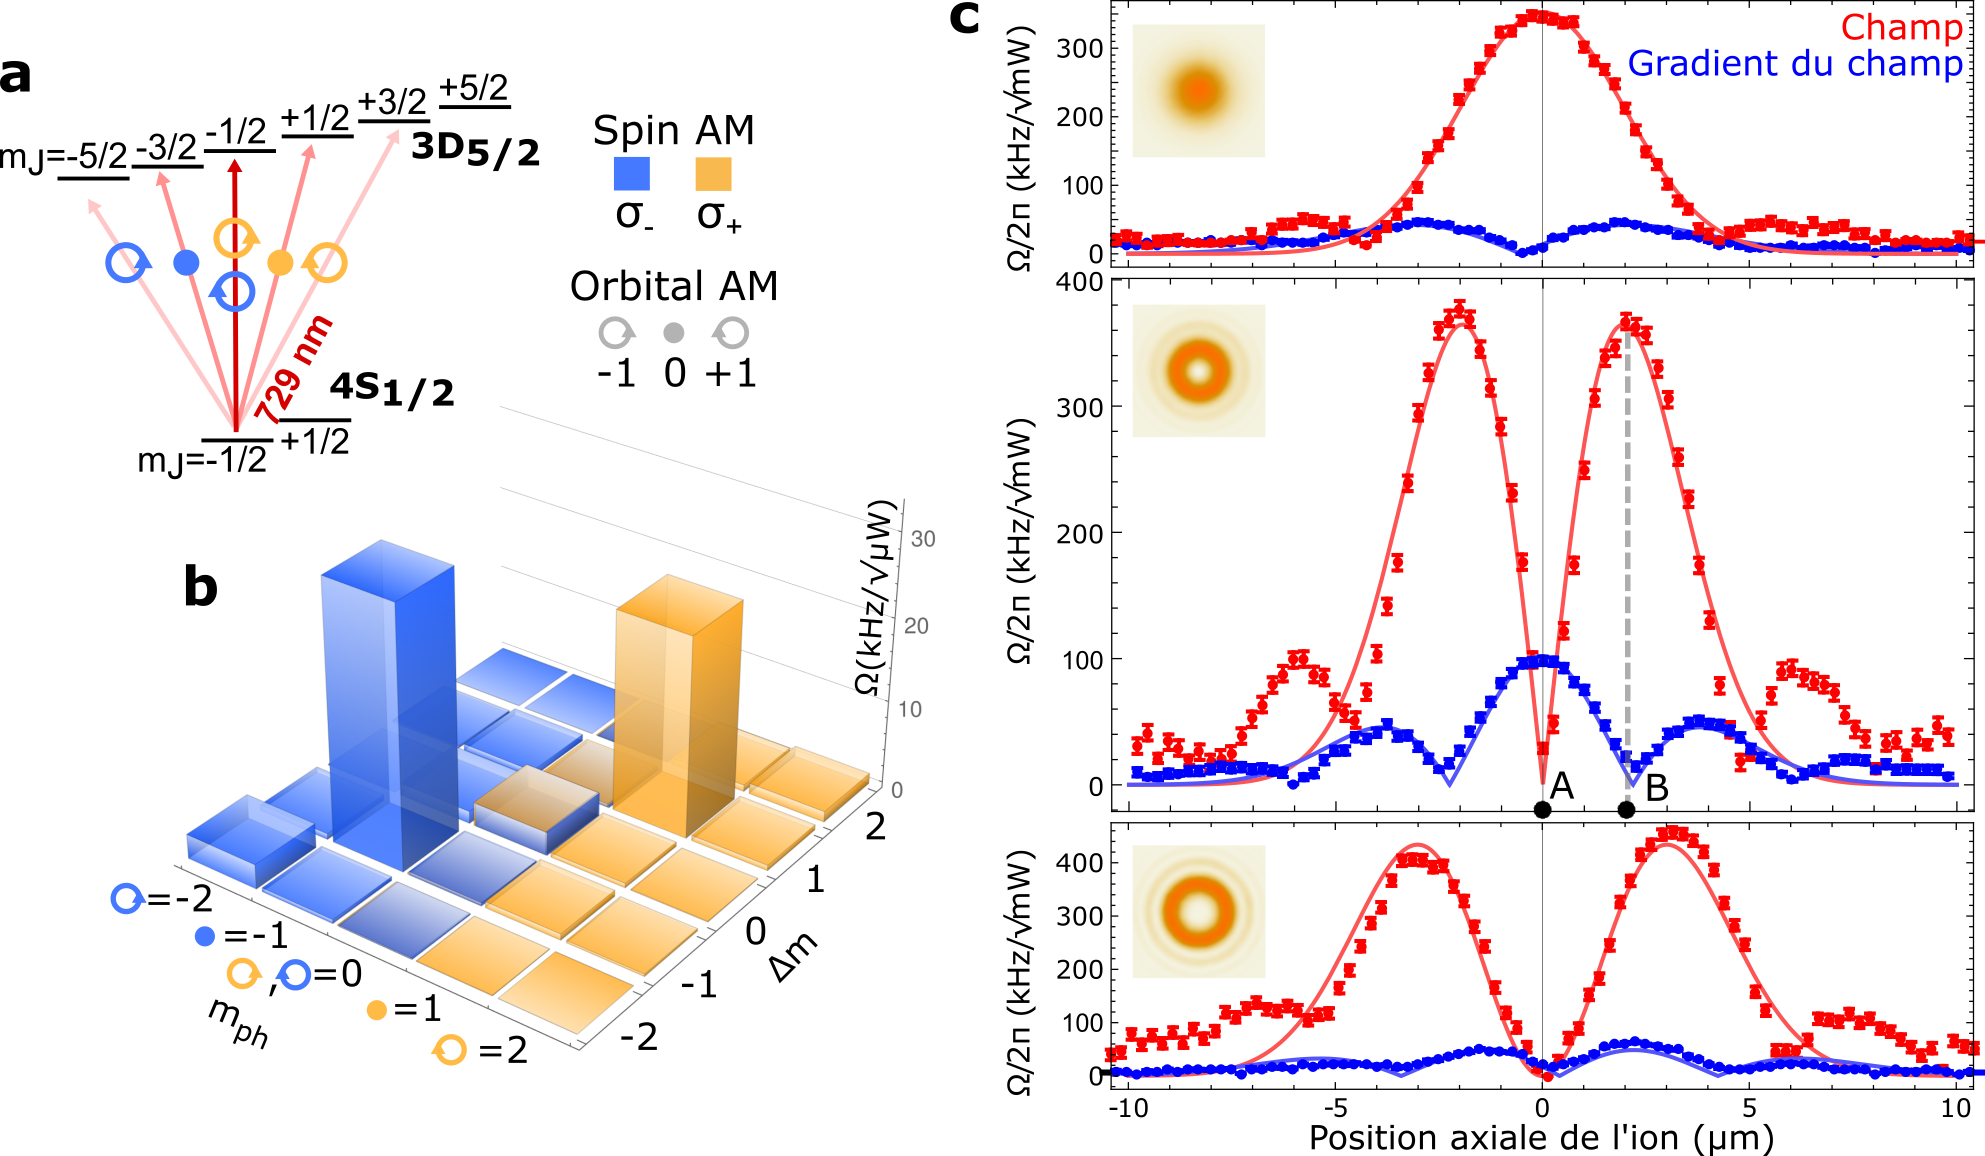
\includegraphics[width=0.9\columnwidth]{Figures/schmiegelow.png}
\caption{Observation de transitions quadripolaires électriques. (a) Transitions possibles mettant en jeu le MAS et le MAO. (b) Amplitudes de transition mesurées en utilisant une oscillation de Rabi. (c) Amplitude de transition dipolaire (rouge) et quadripolaire (bleu) en fonction de la position transverse de l'ion. Ces amplitudes sont reliées respectivement à l'amplitude du champ et du gradient du champ. Tiré de \mycite{schmiegelowarxiv2015}.}
\label{Fig:Schmiegelow}
\end{figure}

\subsubsection{Conclusion de la partie II}
Nous avons introduit les définitions nécessaires et construit des champs électromagnétiques réalisables en pratiques dans lesquelles le moment angulaire est contrôlé. Dans le chapitre III, nous étudierons expérimentalement la génération de modes de Laguerre-Gauss à partir d'un laser infrarouge Gaussien, avant d'utiliser ces modes pour générer des harmoniques d'ordre élevé. Dans le chapitre IV, nous nous intéresserons au cas du moment angulaire de spin, c'est-à-dire de faisceaux polarisés circulairement. Nous chercherons à générer des harmoniques d'ordre élevé polarisées circulairement et à les utiliser dans l'étude de molécules chirales.